\documentclass{FMTslides}
\usepackage[labelformat=simple]{subfig}
\usepackage{tikz}     % For graphics
\usepackage{amsmath, amssymb}  % For various math stuff
\usepackage{subfig}
\usepackage{centernot} % For the centernot macro
%\usepackage{bbding}
\usepackage{groove2tikz}
\usepackage[T1]{fontenc}

% Colours
\newcommand{\red}{red}
\newcommand{\redfill}{\red!10}
\newcommand{\green}{green!75!black}
\newcommand{\greenfill}{\green!10}
\newcommand{\blue}{blue!75!white}
\newcommand{\bluefill}{blue!10}
\newcommand{\grey}{black!8}
\newcommand{\thin}{black!10}
\newcommand{\orange}{orange}
\newcommand{\yellow}{yellow!40}

% Ugly hack to allow nodes with multiple lines
\newcommand{\ml}[1]{
\begin{tabular}{@{}l@{}}#1\vspace{-2pt}\end{tabular}
}

% User specified macro that is run at the end of an exported figure. By
% redefining this macro the user can add more stuff to the figure.
\newcommand{\userdefinedmacro}{\relax}

\usetikzlibrary{arrows, automata, shapes.geometric, positioning, backgrounds}
\DeclareMathAlphabet{\mathitbf}{OML}{cmm}{b}{it}
\input{./commands_style.tex}
% Includes for Tikz
\usetikzlibrary{arrows,automata,positioning,er}

% Dimension styles
\newcommand{\tikzfontsize}{\footnotesize}
\newcommand{\tikzscale}{1.2}
\newcommand{\nodeinsep}{2.5pt}
\newcommand{\labinsep}{2pt}
\renewcommand{\thesubfigure}{\relax} 
\pdfpageattr {/Group << /S /Transparency /I true /CS /DeviceRGB>>}

\title[Model-based Testing with \\Graph Grammars]{Model-based Testing with Graph Grammars}
\conference{\!\!\!M.Sc. Colloquium}
\author{Vincent de Bruijn}
\institute{Formal Methods and Tools, Faculty of EECMS \\ University of Twente, The Netherlands}
\date{April 5th, 2013}

\begin{document}

\maketitleslide

\part{Introduction}

\begin{frame}
   \frametitle{Contents}
   \tableofcontents
\end{frame}

\section{Testing}

\begin{frame}{Testing (1/3)}
\begin{itemize}
  \item Why do we test?
  \begin{itemize}
    \item Products have requirements
    \item Software implementation should uphold requirements
  \end{itemize}
  \begin{center}
    \includegraphics[scale=0.20]{./figures/coffee_machine.jpg}
  \end{center}
\end{itemize}
\end{frame}

\begin{frame}{Testing (2/3)}
\begin{itemize}
  \item Creating tests manually:
  \begin{itemize}
    \item Error-prone
    \item Time intensive
  \end{itemize}
  \begin{center}
    \includegraphics[scale=0.25]{./figures/guy_at_coffee_machine.jpg}
  \end{center}
\end{itemize}
\end{frame}

\begin{frame}{Testing (3/3)}
\begin{itemize}
  \item Solution
  \begin{itemize}
    \item Create `model` from the requirements
    \item Generate tests automatically using model
  \end{itemize}
  \begin{center}
    \includegraphics[scale=0.20]{./figures/abstract_coffee_machine.png}
  \end{center}
\end{itemize}
\end{frame}

\section{Models}

\begin{frame}{Models (1/2)}
\begin{block}{Model}
\begin{itemize}
  \item An abstract representation of the behavior of a system
\end{itemize}
\end{block}
\begin{figure}
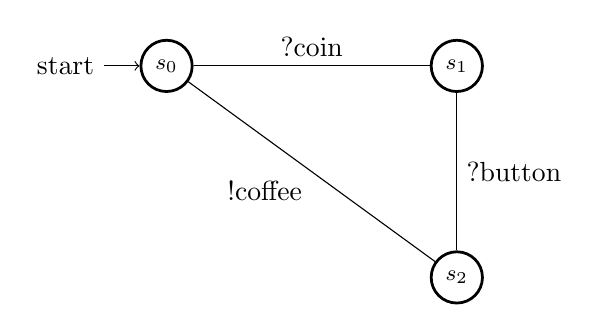
\begin{tikzpicture}
	\tikzstyle{every state}=[draw=black,line width=1pt,fill=white,minimum size=5pt]

	\node[state, initial left] (s0) {\footnotesize $s_0$};
	\node[state] (s1) [right=3cm of s0] {\footnotesize $s_1$};
   	\node[state] (s2) [below=2cm of s1] {\footnotesize $s_2$};
	
	\path        (s0) edge node [auto] {?coin} (s1)
					(s1) edge node [auto] {?button} (s2)
					(s2) edge node [auto] {!coffee} (s0);
\end{tikzpicture}

\end{figure}
\end{frame}

\begin{frame}{Models (2/2)}
\begin{block}{Symbolic Transition System (STS)}
\begin{itemize}
  \item Transition system with \textit{variables}, \textit{constraints} and \textit{updates}
\end{itemize}
\end{block}
\begin{figure}

\usepackage{tikz}     % For graphics
\usepackage{amsmath, amssymb}  % For various math stuff
\usepackage{subfig}
\usepackage{centernot} % For the centernot macro
\usepackage{bbding}

\usetikzlibrary{arrows, automata, shapes.geometric, positioning, backgrounds}

\DeclareMathAlphabet{\mathitbf}{OML}{cmm}{b}{it}

%%%%%%%% COLOURS
\definecolor{darkgreen}{RGB}{0,128,0}


%%%%%%%%%%% HAXXXXORRR

\newenvironment{changemargin}[2]{%
\begin{list}{}{%
\setlength{\topsep}{0pt}%
\setlength{\leftmargin}{#1}%
\setlength{\rightmargin}{#2}%
\setlength{\listparindent}{\parindent}%
\setlength{\itemindent}{\parindent}%
\setlength{\parsep}{\parskip}%
}%
\item[]}{\end{list}}

%%%%%%%%%%%%%%% MATHEMATICAL NOTATIONS%%%%%%%%%
\newcommand{\defi}{\mathrel{{=_{\rm def}}}}
\newcommand{\abs}[1]{\lvert #1 \rvert}
\newcommand{\aut}[1]{\ensuremath{\mathcal{#1}}}
\newcommand{\set}[1]{\{ \, #1 \, \}}
\newcommand{\tuple}[1]{\langle \, #1 \, \rangle}
\newcommand{\suchthat}{\; . \;}
\newcommand{\project}{\mathrel{\upharpoonright}}
\newcommand{\where}{\mid}
\newcommand{\union}{\mathrel{\cup}}
\newcommand{\intersection}{\mathrel{\cap}}
\newcommand{\concat}{\mathrel{\cdot}}
\newcommand{\treq}{\ensuremath{\approx_{\mathrm{tr}} \;}}

\let\oldland\land
\let\oldlor\lor
\let\oldexists\exists
\let\oldforall\forall
\let\oldnexists\nexists

\renewcommand{\land}{\; \oldland \;}
\renewcommand{\lor}{\; \oldlor \;}
\renewcommand{\exists}{\, \oldexists \,}
\renewcommand{\forall}{\, \oldforall \,}
\renewcommand{\nexists}{\, \oldnexists \,}

\newcommand{\existsinfty}{\exists^{\infty}}
\newcommand{\fd}[1]{\ensuremath{\mathit{fd}(#1)}}
\newcommand{\pa}[1]{\ensuremath{\mathit{p}(#1)}}
\newcommand{\qu}[1]{\ensuremath{\mathit{q}(#1)}}
\newcommand{\blockedby}{\nmid}
%%%%%%%%%%%%%%% END MATHEMATICAL NOTATIONS%%%%%%

%%%%%%%%%%%%%%% RULES ETC %%%%%%%%%%%%%%%%%%
\newcounter{ruledefcounter}
\setcounter{ruledefcounter}{1}
\newenvironment{ruledef}[2]%
{\list{}{\leftmargin=0.1in\rightmargin=0in}\item[]\noindent\ignorespaces%
\textbf{Rule R\arabic{ruledefcounter}} %
(#1)%
\textbf{:} %
#2.\list{}{\leftmargin=0.1in\rightmargin=0in}\item[]}
{\endlist\stepcounter{ruledefcounter}\endlist\ignorespacesafterend}
%%%%%%%%%%%%%%% END RULES ETC %%%%%%%%%%%%%%%

%%%%%%%%%%%%%%% THEOREMS ETC %%%%%%%%%%%%%%%
%\theoremstyle{definition}
%\newtheorem{definition}{Definition}[section]
%\theoremstyle{plain}
%\newtheorem{lemma}[definition]{Lemma}
%\newtheorem{proposition}[definition]{Proposition}
%\newtheorem{theorem}[definition]{Theorem}
%\newtheorem{corollary}[definition]{Corollary}
%\theoremstyle{remark}
%\newtheorem{example}[definition]{Example}
%\newtheorem{remark}[definition]{Remark}
%
%\newcommand{\theoremlikeParameterised}[2]{\par\medskip\penalty-250\refstepcounter{definition}{\bfseries\scshape\noindent#1 #2.}\slshape}
%\newenvironment{theoremParam}[1]{\theoremlikeParameterised{\bf Theorem}{#1}}{\par\medskip}
%\newenvironment{lemmaParam}[1]{\theoremlikeParameterised{\bf Lemma}{#1}}{\par\medskip}
%\newenvironment{propositionParam}[1]{\theoremlikeParameterised{\bf Proposition}{#1}}{\par\medskip}
%%%%%%%%%%%%%%% END THEOREMS ETC %%%%%%%%%%%%

%%%%%%%%%%%%%%%% ARROWS %%%%%%%%%%%%%%%%
% auxiliaries
\newcommand{\linefill}{%
   \cleaders
   \hbox{$\smash{\mkern-2mu\mathord-\mkern-2mu}$}%
   \hfill
   \vphantom{\lower1pt\hbox{$\rightarrow$}}%
}

\newcommand{\Linefill}{%
   \cleaders
   \hbox{$\smash{\mkern-2mu\mathord=\mkern-2mu}$}%
   \hfill
   \vphantom{\hbox{$\Rightarrow$}}%
}

% left segment of extensible arrow, no ending
\newcommand{\xleftnoend}[1][]{\mathrel-_{\vphantom{#1}}\mkern-11mu}
\newcommand{\xLeftnoend}[1][]{\mathrel=_{\vphantom{#1}}\mkern-8mu}
% middle segment of extensible arrow
\newcommand{\xmid}[2][]{\stackrel{#2}{\linefill_{\vphantom{#1}}}}
\newcommand{\xMid}[2][]{\stackrel{#2}{\Linefill_{\vphantom{#1}}}}
% right segment of extensible arrow, arrow head
\newcommand{\xrightArrow}[1][]{\mkern-11mu\rightarrow_{#1}}
\newcommand{\xRightArrow}[1][]{\mkern-8mu\Rightarrow_{#1}}
% make arrow symbol
\newcommand{\xmake}[1]{\mathrel{\lower1pt\hbox{$#1$}}}

% single-arrow transition
\newcommand{\trans}[2][]{\xmake{\xleftnoend[#1]\xmid[#1]{#2}\xrightArrow[#1]}}
% negative single-arrow transition
\newcommand{\ntrans}[2][]{\centernot{\trans[#1]{#2}}}
% empty single-arrow transition
\newcommand{\etrans}{\rightarrow}

% double-arrow transition
\newcommand{\Trans}[2][]{\xmake{\xLeftnoend[#1]\xMid[#1]{#2}\xRightArrow[#1]}}
% negative double-arrow transition
\newcommand{\nTrans}[2][]{\centernot{\Trans[#1]{#2}}}
% empty double-arrow transition
\newcommand{\eTrans}{\Rightarrow}
%%%% END ARROWS %%%%%%%%%%%%%%%%%%%%%%%%%

%%%%%%%%%%%%%% TIKZ %%%%%%%%%%%%%%%%
\tikzstyle{background rectangle}= [rounded corners, fill=yellow!20, draw=black, rounded corners=1ex]
\tikzstyle{every picture}=[show background rectangle, ->,>=latex,auto,node distance=1.3cm,thick,initial text=,initial where=above,scale=0.9,transform shape]
\tikzstyle{every state}=[draw=yellow!20,line width=4pt,fill=black,minimum size=5pt]

\tikzstyle{loop right}=[in=-30,out=30,looseness=8]
\tikzstyle{loop left}=[in=150,out=210,looseness=8]
\tikzstyle{loop above}=[in=60,out=120,looseness=8]
\tikzstyle{loop below}=[in=240,out=300,looseness=8]

\tikzstyle{loop above right}=[in=5,out=65,looseness=8]
\tikzstyle{loop above left}=[in=105,out=165,looseness=8]
\tikzstyle{loop slightly above left}=[in=125,out=185,looseness=8]
\tikzstyle{loop slightly above right}=[in=5,out=65,looseness=8]
\tikzstyle{loop below left}=[in=195,out=255,looseness=8]
\tikzstyle{loop below right}=[in=285,out=-15,looseness=8]
\tikzstyle{loop slightly below left}=[in=155,out=215,looseness=8]
\tikzstyle{loop slightly below right}=[in=305,out=5,looseness=8]

\tikzstyle{nodeSmall} = [state, node distance=1.5cm, draw=yellow!20, fill=black]
\tikzstyle{finalNode} = [node distance=1.5cm]
\newcommand{\back}{\color{yellow!20}mm}
\tikzstyle{onEdge}=[fill=yellow!20, pos=0.5]
%%%%%%%%%%%%%% END TIKZ %%%%%%%%%%%%%

%%%%%%%%%%%%%% USEFUL ALIASES %%%%%%%%%
\newcommand{\ioco}{\texttt{ioco}}

\newcommand{\impl}{\aut{A}_i}
\newcommand{\spec}{\aut{A}_s}
\newcommand{\ioconf}{\sqsubseteq_{\ioco}}

\newcommand{\AparB}{\ensuremath{\aut{A} \parallel \aut{B}}}
\newcommand{\AparBie}{\ensuremath{\aut{A} \parallel_{\rm I} \aut{B}}}

\newcommand{\Lin}{L^{\text{\rm I}}}
\newcommand{\Lout}{L^{\text{\rm O}}}
\newcommand{\Ltau}{L^{\tau}}
\newcommand{\Ldelta}{L^{\delta}}
\newcommand{\Ltaudelta}{L^{\delta}_{\tau}}
\newcommand{\LA}{L_{\aut{A}}}
\newcommand{\LB}{L_{\aut{B}}}
\newcommand{\LC}{L_{\aut{C}}}
\newcommand{\LD}{L_{\aut{D}}}
\newcommand{\LinA}{\Lin_{\aut{A}}}
\newcommand{\LinB}{\Lin_{\aut{B}}}
\newcommand{\LinC}{\Lin_{\aut{C}}}
\newcommand{\LinD}{\Lin_{\aut{D}}}
\newcommand{\LoutA}{\Lout_{\aut{A}}}
\newcommand{\LoutB}{\Lout_{\aut{B}}}
\newcommand{\LoutC}{\Lout_{\aut{C}}}
\newcommand{\LoutD}{\Lout_{\aut{D}}}
\newcommand{\LoutHide}{\Lout_{H}}
\newcommand{\LtauA}{\Ltau_{\aut{A}}}
\newcommand{\LtauB}{\Ltau_{\aut{B}}}
\newcommand{\LtauC}{\Ltau_{\aut{C}}}
\newcommand{\LtauD}{\Ltau_{\aut{D}}}
\newcommand{\LtauHide}{\Ltau_{H}}
\newcommand{\LdeltaA}{\Ldelta_{\aut{A}}}
\newcommand{\LdeltaB}{\Ldelta_{\aut{B}}}
\newcommand{\LdeltaC}{\Ldelta_{\aut{C}}}
\newcommand{\LdeltaD}{\Ldelta_{\aut{D}}}
\newcommand{\LAparB}{L_{\AparB}}
\newcommand{\LinAparB}{\Lin_{\AparB}}
\newcommand{\LoutAparB}{\Lout_{\AparB}}
\newcommand{\LtauAparB}{\Ltau_{\AparB}}
\newcommand{\LdeltaAparB}{\Ldelta_{\AparB}}

\newcommand{\sdelta}{s_{\delta}}
\newcommand{\fdelta}{f_{\delta}}

\newcommand{\SA}{S_{\aut{A}}}
\newcommand{\SB}{S_{\aut{B}}}
\newcommand{\SC}{S_{\aut{C}}}
\newcommand{\SD}{S_{\aut{D}}}
\newcommand{\SAparB}{S_{\AparB}}
\newcommand{\Sdelta}{S_{\delta}}
\newcommand{\Shide}{S_{H}}

\newcommand{\Sstart}{S^0}
\newcommand{\SstartA}{\Sstart_{\aut{A}}}
\newcommand{\SstartB}{\Sstart_{\aut{B}}}
\newcommand{\SstartC}{\Sstart_{\aut{C}}}
\newcommand{\SstartD}{\Sstart_{\aut{D}}}
\newcommand{\SstartAparB}{\Sstart_{\AparB}}

\newcommand{\PA}{P_{\aut{A}}}
\newcommand{\PB}{P_{\aut{B}}}
\newcommand{\PC}{P_{\aut{C}}}
\newcommand{\PD}{P_{\aut{D}}}
\newcommand{\PAparB}{P_{\AparB}}

\newcommand{\transA}[2][]{\trans[#1]{#2}_{\aut{A}}}
\newcommand{\transB}[2][]{\trans[#1]{#2}_{\aut{B}}}
\newcommand{\transC}[2][]{\trans[#1]{#2}_{\aut{C}}}
\newcommand{\transD}[2][]{\trans[#1]{#2}_{\aut{D}}}
\newcommand{\transAparB}[2][]{\trans[#1]{#2}_{\AparB}}
\newcommand{\transAparBie}[2][]{\trans[#1]{#2}_{\AparBie}}
\newcommand{\transDelta}[2][]{\trans[#1]{#2}_{\delta}}
\newcommand{\transDet}[2][]{\trans[#1]{#2}_{\mathrm{D}}}
\newcommand{\transHide}[2][]{\trans[#1]{#2}_{H}}
\newcommand{\transDeltaHide}[2][]{\trans[#1]{#2}_{\delta(\mathrm{H})}}
\newcommand{\transHideDelta}[2][]{\trans[#1]{#2}_{\mathrm{H}(\delta)}}

\newcommand{\TransA}[2][]{\Trans[#1]{#2}_{\aut{A}}}
\newcommand{\TransB}[2][]{\Trans[#1]{#2}_{\aut{B}}}
\newcommand{\TransC}[2][]{\Trans[#1]{#2}_{\aut{C}}}
\newcommand{\TransD}[2][]{\Trans[#1]{#2}_{\aut{D}}}
\newcommand{\TransAparB}[2][]{\Trans[#1]{#2}_{\AparB}}
\newcommand{\TransAparBie}[2][]{\Trans[#1]{#2}_{\AparBie}}
\newcommand{\TransDelta}[2][]{\Trans[#1]{#2}_{\delta}}
\newcommand{\TransDet}[2][]{\Trans[#1]{#2}_{\mathrm{D}}}
\newcommand{\TransHide}[2][]{\Trans[#1]{#2}_{H}}
\newcommand{\TransHideDelta}[2][]{\Trans[#1]{#2}_{\mathrm{H}(\delta)}}

\newcommand{\ntransA}[2][]{\ntrans[#1]{#2}_{\aut{A}}}
\newcommand{\ntransB}[2][]{\ntrans[#1]{#2}_{\aut{B}}}
\newcommand{\ntransC}[2][]{\ntrans[#1]{#2}_{\aut{C}}}
\newcommand{\ntransD}[2][]{\ntrans[#1]{#2}_{\aut{D}}}
\newcommand{\ntransAparB}[2][]{\ntrans[#1]{#2}_{\AparB}}
\newcommand{\ntransAparBie}[2][]{\ntrans[#1]{#2}_{\AparBie}}
\newcommand{\ntransDelta}[2][]{\ntrans[#1]{#2}_{\delta}}
\newcommand{\ntransHide}[2][]{\ntrans[#1]{#2}_{H}}
\newcommand{\ntransDet}[2][]{\ntrans[#1]{#2}_{\mathrm{D}}}

\newcommand{\nTransA}[2][]{\nTrans[#1]{#2}_{\aut{A}}}
\newcommand{\nTransB}[2][]{\nTrans[#1]{#2}_{\aut{B}}}
\newcommand{\nTransC}[2][]{\nTrans[#1]{#2}_{\aut{C}}}
\newcommand{\nTransD}[2][]{\nTrans[#1]{#2}_{\aut{D}}}
\newcommand{\nTransAparB}[2][]{\nTrans[#1]{#2}_{\AparB}}
\newcommand{\nTransAparBie}[2][]{\nTrans[#1]{#2}_{\AparBie}}
\newcommand{\nTransDelta}[2][]{\nTrans[#1]{#2}_{\delta}}
\newcommand{\nTransDet}[2][]{\nTrans[#1]{#2}_{\mathrm{D}}}
\newcommand{\nTransHide}[2][]{\nTrans[#1]{#2}_{H}}

\newcommand{\etransA}{\etrans_{\aut{A}}}
\newcommand{\etransB}{\etrans_{\aut{B}}}
\newcommand{\etransC}{\etrans_{\aut{C}}}
\newcommand{\etransD}{\etrans_{\aut{D}}}
\newcommand{\etransAparB}{\etrans_{\AparB}}
\newcommand{\etransAparBie}{\etrans_{\AparBie}}
\newcommand{\etransDelta}{\etrans_{\delta}}
\newcommand{\etransDet}{\etrans_{\mathrm{D}}}
\newcommand{\etransHide}{\etrans_{H}}
\newcommand{\etransDeltaHide}{\etrans_{\delta(\mathrm{H})}}
\newcommand{\etransHideDelta}{\etrans_{\mathrm{H}(\delta)}}

\newcommand{\deltaf}[1]{\ensuremath{\delta(#1)}}
\newcommand{\deter}[1]{\ensuremath{\mathit{det}(#1)}}
\newcommand{\hide}[2]{\ensuremath{#1 \setminus #2}}
\newcommand{\init}[1]{\ensuremath{\mathit{init}(#1)}}
\newcommand{\trace}[1]{\ensuremath{\mathit{trace}(#1)}}
\newcommand{\states}[1]{\ensuremath{\mathit{states}(#1)}}
\newcommand{\paths}[1]{\ensuremath{\mathit{paths}(#1)}}
\newcommand{\dpaths}[1]{\ensuremath{\mathit{dpaths}(#1)}}
\newcommand{\fpaths}[1]{\ensuremath{\mathit{fpaths}(#1)}}
\newcommand{\fdpaths}[1]{\ensuremath{\mathit{fdpaths}(#1)}}

\newcommand{\rs}[1]{\ensuremath{\mathit{rs}_{#1}}}
\newcommand{\qos}[1]{\ensuremath{\mathit{qos}_{#1}}}

\newcommand{\fdclosures}[1]{\ensuremath{\mathit{fdclosures}(#1)}}
\newcommand{\newfdclosures}[1]{\ensuremath{\mathit{new\text{-}fdclosures}(#1)}}

\newcommand{\reach}[1]{\ensuremath{\mathit{reach}(#1)}}
\newcommand{\reachA}[1]{\ensuremath{\mathit{reach}_{\aut{A}}(#1)}}
\newcommand{\reachB}[1]{\ensuremath{\mathit{reach}_{\aut{B}}(#1)}}
\newcommand{\reachAparB}[1]{\ensuremath{\mathit{reach}_{\AparB}(#1)}}
\newcommand{\reachHide}[1]{\ensuremath{\mathit{reach}_{H}(#1)}}

\newcommand{\traces}[1]{\ensuremath{\mathit{traces}(#1)}}
\newcommand{\tracesA}[1]{\ensuremath{\mathit{traces}_{\aut{A}}(#1)}}
\newcommand{\tracesB}[1]{\ensuremath{\mathit{traces}_{\aut{B}}(#1)}}
\newcommand{\tracesAparB}[1]{\ensuremath{\mathit{traces}_{\AparB}(#1)}}
\newcommand{\tracesDelta}[1]{\ensuremath{\mathit{traces}_{\delta}(#1)}}
\newcommand{\tracesDet}[1]{\ensuremath{\mathit{traces}_{\mathrm{D}}(#1)}}
\newcommand{\tracesHide}[1]{\ensuremath{\mathit{traces}_{H}(#1)}}
\newcommand{\tracesDeltaHide}[1]{\ensuremath{\mathit{traces}_{\delta(\mathrm{H})}(#1)}}
\newcommand{\tracesHideDelta}[1]{\ensuremath{\mathit{traces}_{\mathrm{H}(\delta)}(#1)}}
%%%%%%%%%%% END USEFUL ALIASES  %%%%%%%%%

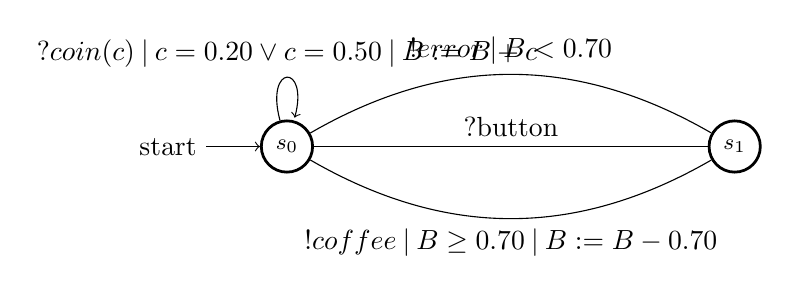
\begin{tikzpicture}[scale=1.5]
	\tikzstyle{every state}=[draw=black,line width=1pt,fill=white,minimum size=5pt]

	\node[state, initial left] (s0) {\footnotesize $s_0$};
	\node[state] (s1) [right=5cm of s0] {\footnotesize $s_1$};
	
	\path (s0) edge[min distance=20mm,loop above] node [auto] {$?coin(c)\:|\:c=0.20 \lor c=0.50\:|\:B:=B+c$ } (s0) ;
	\path (s0) edge node [auto] {?button} (s1) ;
	\path (s1) edge[out=210,in=-30] node [auto] {$!coffee\:|\:B\geq 0.70\:|\:B:=B-0.70$} (s0) ;
  \path (s1) edge[out=150,in=30] node [above] {$!error\:|\:B<0.70$} (s0) ;
\end{tikzpicture}

\end{figure}
\end{frame}

\section{Model-based Testing}

\begin{frame}{Model-based Testing (1/1)}
\begin{figure}
\tikzstyle every node=[scale=\tikzscale*0.5,font=\tikzfontsize\sffamily,inner sep=\nodeinsep,minimum size=9pt,rounded corners=1pt]

% LTS colours
\tikzstyle{result}=[fill=orange]
\tikzstyle{final}=[fill=red]
\tikzstyle{start}=[fill=green]
\tikzstyle{open}=[fill=black!40]

% Readers
\tikzstyle{node}=[draw=black,fill=\grey,shape=rectangle]
\tikzstyle{edge}=[draw,black,-stealth']
\tikzstyle{lab}=[fill=white,inner sep=\labinsep]

% Erasers
\tikzstyle{delnode}=[draw=\blue,fill=\bluefill,text=\blue,shape=rectangle,densely dashed]
\tikzstyle{deledge}=[draw,\blue,densely dashed,-stealth']
\tikzstyle{dellab}=[text=\blue,fill=white,inner sep=\labinsep]

% Creators
\tikzstyle{newnode}=[draw=\green,fill=\greenfill,very thick,text=\green,shape=rectangle]
\tikzstyle{newedge}=[draw,\green,very thick,-stealth']
\tikzstyle{newlab}=[text=\green,fill=white,inner sep=\labinsep]

% NACs
\tikzstyle{nacnode}=[draw=\red,fill=\redfill,text=\red,line width=2pt,dotted,shape=rectangle]
\tikzstyle{nacedge}=[draw,\red,line width=2pt,dotted,-stealth']
\tikzstyle{naclab}=[text=\red,fill=white,inner sep=\labinsep]

% Remarks
\tikzstyle{remnode}=[draw=\orange,fill=\yellow,text=\orange,shape=rectangle]
\tikzstyle{remedge}=[draw,\orange,-stealth']
\tikzstyle{remlab}=[text=\orange,fill=white,inner sep=\labinsep]

% Quantifiers
\tikzstyle{quantnode}=[draw=black,dotted,fill=\grey,shape=rectangle]
\tikzstyle{quantedge}=[draw,black,dotted,-stealth']

% Parameter nodes
\tikzstyle{parnode}=[draw=black,fill=black,text=white,shape=rectangle,font=\scriptsize\sffamily,inner sep=1pt,minimum size=4pt,anchor=east]

% Special styles (can be combined with the above)
\tikzstyle{attr}=[shape=ellipse,inner sep=1pt]
\tikzstyle{prod}=[shape=diamond,inner sep=1pt,shape aspect=2]
\tikzstyle{whitefill}=[fill=white]
\tikzstyle{bold}=[very thick]
\tikzstyle{ultrabold}=[line width=2pt]
\tikzstyle{thinnode}=[draw=\thin,text=\thin,fill=white,shape=rectangle]
\tikzstyle{thinedge}=[draw,\thin,text=\thin,-stealth']
\tikzstyle{thinlab}=[text=\thin,fill=white,inner sep=\labinsep]
\tikzstyle{type}=[rounded corners=0pt]
\tikzstyle{bidir}=[stealth'-stealth']

% Abstract types
\tikzstyle{absnode}=[draw=black,fill=\grey,shape=rectangle,densely dashed]
\tikzstyle{absedge}=[draw,black,-stealth',densely dashed]
\tikzstyle{abslab}=[font=\tikzfontsize\sffamily\slshape,fill=white,inner sep=\labinsep]

% Inheritance edge
\tikzstyle{subedge}=[draw,->,>=open triangle 60]

% Composite edge
\tikzstyle{partedge}=[draw,diamond->]

% Multiplicity labels
\tikzstyle{inmultlab}=[lab,auto=left,very near start]
\tikzstyle{outmultlab}=[lab,auto=left,very near end]

% Nodified edges
\tikzstyle{nodified}=[draw=black,fill=white,shape=circle,inner sep=0pt,minimum size=4pt]

% Control automaton
%  Nodes
\tikzstyle{cnode}=[draw=black,fill=\grey,shape=rectangle]
\tikzstyle{cstart}=[draw=black,fill=green,shape=rectangle]
\tikzstyle{csuccess}=[draw=black,fill=red,shape=rectangle]
%  Edges
\tikzstyle{cedge}=[draw,black,-stealth']
\tikzstyle{clambda}=[draw,green,-stealth']
\tikzstyle{cfailure}=[draw,red,-stealth']
%  Labels
\tikzstyle{clab}=[black,fill=white,inner sep=\labinsep]


\begin{tikzpicture}
\node (Model) {
  \includegraphics[scale=0.20]{./figures/coffee_pic.png}
};
\node (SUT) [right=5cm of Model] {
  \includegraphics[scale=0.10]{./figures/coffee_machine.jpg}
};

\path ([yshift=2ex]Model.east) edge[-triangle 60] node [above] {input} ([yshift=2ex]SUT.west) ;
\path ([yshift=-2ex]SUT.west) edge[-triangle 60] node [below] {output}  ([yshift=-2ex]Model.east) ;
\end{tikzpicture}
\end{figure}
\begin{enumerate}
\item Take possible stimulus from model
\item Apply stimulus to SUT
\item Observe response(s)
\item Check if according to model
\item Notify tester whether test passed or failed
\end{enumerate}
\end{frame}

\section{Graph Grammars}

\begin{frame}{Graph Grammars (1/3)}
\begin{figure}
\centering
% To use this figure in your LaTeX document
% import the package groove/resources/groove2tikz.sty
%
% Special colors
\begin{tikzpicture}[
% Special color styles
scale=\tikzscale]
\node[node] (n6)  at (2.705, -1.305) {\ml{Coffee}};
\node[node] (n2)  at (2.685, -0.705) {\ml{Button}};
\node[node] (n0)  at (1.160, -0.695) {\ml{CoffeeMachine}};
\path[edge](n0.east |- 2.685, -0.705) -- node[lab]{has} (n2) ;
\path[edge](n2.south -| 2.705, -1.305) -- node[lab]{for} (n6) ;
\userdefinedmacro
\end{tikzpicture}
\renewcommand{\userdefinedmacro}{\relax}

\end{figure}

\begin{itemize}
  \item Graphs represent system states
  \item Graph rules express possible changes to graph
  \item All possible changes make a \textit{Graph Transition System}
\end{itemize}
\end{frame}

\begin{frame}{Graph Grammars (2/3)}
\begin{figure}
\centering
  \subfloat[?coin]{% To use this figure in your LaTeX document
% import the package groove/resources/groove2tikz.sty
%
% Special colors
%\tikzstyle every node=[scale=\tikzscale*0.5,font=\tikzfontsize\sffamily,inner sep=\nodeinsep,minimum size=9pt,rounded corners=1pt]

% LTS colours
\tikzstyle{result}=[fill=orange]
\tikzstyle{final}=[fill=red]
\tikzstyle{start}=[fill=green]
\tikzstyle{open}=[fill=black!40]

% Readers
\tikzstyle{node}=[draw=black,fill=\grey,shape=rectangle]
\tikzstyle{edge}=[draw,black,-stealth']
\tikzstyle{lab}=[fill=white,inner sep=\labinsep]

% Erasers
\tikzstyle{delnode}=[draw=\blue,fill=\bluefill,text=\blue,shape=rectangle,densely dashed]
\tikzstyle{deledge}=[draw,\blue,densely dashed,-stealth']
\tikzstyle{dellab}=[text=\blue,fill=white,inner sep=\labinsep]

% Creators
\tikzstyle{newnode}=[draw=\green,fill=\greenfill,very thick,text=\green,shape=rectangle]
\tikzstyle{newedge}=[draw,\green,very thick,-stealth']
\tikzstyle{newlab}=[text=\green,fill=white,inner sep=\labinsep]

% NACs
\tikzstyle{nacnode}=[draw=\red,fill=\redfill,text=\red,line width=2pt,dotted,shape=rectangle]
\tikzstyle{nacedge}=[draw,\red,line width=2pt,dotted,-stealth']
\tikzstyle{naclab}=[text=\red,fill=white,inner sep=\labinsep]

% Remarks
\tikzstyle{remnode}=[draw=\orange,fill=\yellow,text=\orange,shape=rectangle]
\tikzstyle{remedge}=[draw,\orange,-stealth']
\tikzstyle{remlab}=[text=\orange,fill=white,inner sep=\labinsep]

% Quantifiers
\tikzstyle{quantnode}=[draw=black,dotted,fill=\grey,shape=rectangle]
\tikzstyle{quantedge}=[draw,black,dotted,-stealth']

% Parameter nodes
\tikzstyle{parnode}=[draw=black,fill=black,text=white,shape=rectangle,font=\scriptsize\sffamily,inner sep=1pt,minimum size=4pt,anchor=east]

% Special styles (can be combined with the above)
\tikzstyle{attr}=[shape=ellipse,inner sep=1pt]
\tikzstyle{prod}=[shape=diamond,inner sep=1pt,shape aspect=2]
\tikzstyle{whitefill}=[fill=white]
\tikzstyle{bold}=[very thick]
\tikzstyle{ultrabold}=[line width=2pt]
\tikzstyle{thinnode}=[draw=\thin,text=\thin,fill=white,shape=rectangle]
\tikzstyle{thinedge}=[draw,\thin,text=\thin,-stealth']
\tikzstyle{thinlab}=[text=\thin,fill=white,inner sep=\labinsep]
\tikzstyle{type}=[rounded corners=0pt]
\tikzstyle{bidir}=[stealth'-stealth']

% Abstract types
\tikzstyle{absnode}=[draw=black,fill=\grey,shape=rectangle,densely dashed]
\tikzstyle{absedge}=[draw,black,-stealth',densely dashed]
\tikzstyle{abslab}=[font=\tikzfontsize\sffamily\slshape,fill=white,inner sep=\labinsep]

% Inheritance edge
\tikzstyle{subedge}=[draw,->,>=open triangle 60]

% Composite edge
\tikzstyle{partedge}=[draw,diamond->]

% Multiplicity labels
\tikzstyle{inmultlab}=[lab,auto=left,very near start]
\tikzstyle{outmultlab}=[lab,auto=left,very near end]

% Nodified edges
\tikzstyle{nodified}=[draw=black,fill=white,shape=circle,inner sep=0pt,minimum size=4pt]

% Control automaton
%  Nodes
\tikzstyle{cnode}=[draw=black,fill=\grey,shape=rectangle]
\tikzstyle{cstart}=[draw=black,fill=green,shape=rectangle]
\tikzstyle{csuccess}=[draw=black,fill=red,shape=rectangle]
%  Edges
\tikzstyle{cedge}=[draw,black,-stealth']
\tikzstyle{clambda}=[draw,green,-stealth']
\tikzstyle{cfailure}=[draw,red,-stealth']
%  Labels
\tikzstyle{clab}=[black,fill=white,inner sep=\labinsep]

\begin{tikzpicture}[
% Special color styles
scale=\tikzscale]
\node[newnode] (n0)  at (0.990, -0.685) {\ml{Coin}};
\node[node] (n1)  at (2.310, -0.685) {\ml{CoffeeMachine}};
\node[nacnode] (n2)  at (0.980, -1.295) {\ml{Coin}};
\path[newedge](n0.east |- 2.310, -0.685) -- node[newlab]{in} (n1) ;
\path[nacedge] (n2)  -- node[naclab]{in} (n1) ;
\userdefinedmacro
\end{tikzpicture}
\renewcommand{\userdefinedmacro}{\relax}
}\hspace{10px}
  \subfloat[?button]{% To use this figure in your LaTeX document
% import the package groove/resources/groove2tikz.sty
%
% Special colors
%\tikzstyle every node=[scale=\tikzscale*0.5,font=\tikzfontsize\sffamily,inner sep=\nodeinsep,minimum size=9pt,rounded corners=1pt]

% LTS colours
\tikzstyle{result}=[fill=orange]
\tikzstyle{final}=[fill=red]
\tikzstyle{start}=[fill=green]
\tikzstyle{open}=[fill=black!40]

% Readers
\tikzstyle{node}=[draw=black,fill=\grey,shape=rectangle]
\tikzstyle{edge}=[draw,black,-stealth']
\tikzstyle{lab}=[fill=white,inner sep=\labinsep]

% Erasers
\tikzstyle{delnode}=[draw=\blue,fill=\bluefill,text=\blue,shape=rectangle,densely dashed]
\tikzstyle{deledge}=[draw,\blue,densely dashed,-stealth']
\tikzstyle{dellab}=[text=\blue,fill=white,inner sep=\labinsep]

% Creators
\tikzstyle{newnode}=[draw=\green,fill=\greenfill,very thick,text=\green,shape=rectangle]
\tikzstyle{newedge}=[draw,\green,very thick,-stealth']
\tikzstyle{newlab}=[text=\green,fill=white,inner sep=\labinsep]

% NACs
\tikzstyle{nacnode}=[draw=\red,fill=\redfill,text=\red,line width=2pt,dotted,shape=rectangle]
\tikzstyle{nacedge}=[draw,\red,line width=2pt,dotted,-stealth']
\tikzstyle{naclab}=[text=\red,fill=white,inner sep=\labinsep]

% Remarks
\tikzstyle{remnode}=[draw=\orange,fill=\yellow,text=\orange,shape=rectangle]
\tikzstyle{remedge}=[draw,\orange,-stealth']
\tikzstyle{remlab}=[text=\orange,fill=white,inner sep=\labinsep]

% Quantifiers
\tikzstyle{quantnode}=[draw=black,dotted,fill=\grey,shape=rectangle]
\tikzstyle{quantedge}=[draw,black,dotted,-stealth']

% Parameter nodes
\tikzstyle{parnode}=[draw=black,fill=black,text=white,shape=rectangle,font=\scriptsize\sffamily,inner sep=1pt,minimum size=4pt,anchor=east]

% Special styles (can be combined with the above)
\tikzstyle{attr}=[shape=ellipse,inner sep=1pt]
\tikzstyle{prod}=[shape=diamond,inner sep=1pt,shape aspect=2]
\tikzstyle{whitefill}=[fill=white]
\tikzstyle{bold}=[very thick]
\tikzstyle{ultrabold}=[line width=2pt]
\tikzstyle{thinnode}=[draw=\thin,text=\thin,fill=white,shape=rectangle]
\tikzstyle{thinedge}=[draw,\thin,text=\thin,-stealth']
\tikzstyle{thinlab}=[text=\thin,fill=white,inner sep=\labinsep]
\tikzstyle{type}=[rounded corners=0pt]
\tikzstyle{bidir}=[stealth'-stealth']

% Abstract types
\tikzstyle{absnode}=[draw=black,fill=\grey,shape=rectangle,densely dashed]
\tikzstyle{absedge}=[draw,black,-stealth',densely dashed]
\tikzstyle{abslab}=[font=\tikzfontsize\sffamily\slshape,fill=white,inner sep=\labinsep]

% Inheritance edge
\tikzstyle{subedge}=[draw,->,>=open triangle 60]

% Composite edge
\tikzstyle{partedge}=[draw,diamond->]

% Multiplicity labels
\tikzstyle{inmultlab}=[lab,auto=left,very near start]
\tikzstyle{outmultlab}=[lab,auto=left,very near end]

% Nodified edges
\tikzstyle{nodified}=[draw=black,fill=white,shape=circle,inner sep=0pt,minimum size=4pt]

% Control automaton
%  Nodes
\tikzstyle{cnode}=[draw=black,fill=\grey,shape=rectangle]
\tikzstyle{cstart}=[draw=black,fill=green,shape=rectangle]
\tikzstyle{csuccess}=[draw=black,fill=red,shape=rectangle]
%  Edges
\tikzstyle{cedge}=[draw,black,-stealth']
\tikzstyle{clambda}=[draw,green,-stealth']
\tikzstyle{cfailure}=[draw,red,-stealth']
%  Labels
\tikzstyle{clab}=[black,fill=white,inner sep=\labinsep]

\begin{tikzpicture}[
% Special color styles
scale=\tikzscale]
\node[node] (n5)  at (0.960, -0.675) {\ml{Coin}};
\node[nacnode] (n4)  at (3.625, -0.690) {\ml{\textit{pushed}\\Button}};
\node[node] (n3)  at (3.625, -1.485) {\ml{Coffee}};
\node[node] (n0)  at (2.240, -1.480) {\ml{{\color{\green}\textit{$+$ pushed}}\\Button}};
\node[node] (n1)  at (2.240, -0.675) {\ml{CoffeeMachine}};
\path[edge](n5.east |- 2.240, -0.675) -- node[lab]{in} (n1) ;
\path[nacedge](n1.east |- 3.625, -0.690) -- node[naclab]{has} (n4) ;
\path[edge](n0.east |- 3.625, -1.485) -- node[lab]{for} (n3) ;
\path[edge](n1.south -| 2.240, -1.480) -- node[lab]{has} (n0) ;
\path[nacedge](n4.south -| 3.625, -1.485) -- node[naclab]{for} (n3) ;
\userdefinedmacro
\end{tikzpicture}
\renewcommand{\userdefinedmacro}{\relax}
}\\
  \subfloat[!coffee]{% To use this figure in your LaTeX document
% import the package groove/resources/groove2tikz.sty
%
% Special colors
%\tikzstyle every node=[scale=\tikzscale*0.5,font=\tikzfontsize\sffamily,inner sep=\nodeinsep,minimum size=9pt,rounded corners=1pt]

% LTS colours
\tikzstyle{result}=[fill=orange]
\tikzstyle{final}=[fill=red]
\tikzstyle{start}=[fill=green]
\tikzstyle{open}=[fill=black!40]

% Readers
\tikzstyle{node}=[draw=black,fill=\grey,shape=rectangle]
\tikzstyle{edge}=[draw,black,-stealth']
\tikzstyle{lab}=[fill=white,inner sep=\labinsep]

% Erasers
\tikzstyle{delnode}=[draw=\blue,fill=\bluefill,text=\blue,shape=rectangle,densely dashed]
\tikzstyle{deledge}=[draw,\blue,densely dashed,-stealth']
\tikzstyle{dellab}=[text=\blue,fill=white,inner sep=\labinsep]

% Creators
\tikzstyle{newnode}=[draw=\green,fill=\greenfill,very thick,text=\green,shape=rectangle]
\tikzstyle{newedge}=[draw,\green,very thick,-stealth']
\tikzstyle{newlab}=[text=\green,fill=white,inner sep=\labinsep]

% NACs
\tikzstyle{nacnode}=[draw=\red,fill=\redfill,text=\red,line width=2pt,dotted,shape=rectangle]
\tikzstyle{nacedge}=[draw,\red,line width=2pt,dotted,-stealth']
\tikzstyle{naclab}=[text=\red,fill=white,inner sep=\labinsep]

% Remarks
\tikzstyle{remnode}=[draw=\orange,fill=\yellow,text=\orange,shape=rectangle]
\tikzstyle{remedge}=[draw,\orange,-stealth']
\tikzstyle{remlab}=[text=\orange,fill=white,inner sep=\labinsep]

% Quantifiers
\tikzstyle{quantnode}=[draw=black,dotted,fill=\grey,shape=rectangle]
\tikzstyle{quantedge}=[draw,black,dotted,-stealth']

% Parameter nodes
\tikzstyle{parnode}=[draw=black,fill=black,text=white,shape=rectangle,font=\scriptsize\sffamily,inner sep=1pt,minimum size=4pt,anchor=east]

% Special styles (can be combined with the above)
\tikzstyle{attr}=[shape=ellipse,inner sep=1pt]
\tikzstyle{prod}=[shape=diamond,inner sep=1pt,shape aspect=2]
\tikzstyle{whitefill}=[fill=white]
\tikzstyle{bold}=[very thick]
\tikzstyle{ultrabold}=[line width=2pt]
\tikzstyle{thinnode}=[draw=\thin,text=\thin,fill=white,shape=rectangle]
\tikzstyle{thinedge}=[draw,\thin,text=\thin,-stealth']
\tikzstyle{thinlab}=[text=\thin,fill=white,inner sep=\labinsep]
\tikzstyle{type}=[rounded corners=0pt]
\tikzstyle{bidir}=[stealth'-stealth']

% Abstract types
\tikzstyle{absnode}=[draw=black,fill=\grey,shape=rectangle,densely dashed]
\tikzstyle{absedge}=[draw,black,-stealth',densely dashed]
\tikzstyle{abslab}=[font=\tikzfontsize\sffamily\slshape,fill=white,inner sep=\labinsep]

% Inheritance edge
\tikzstyle{subedge}=[draw,->,>=open triangle 60]

% Composite edge
\tikzstyle{partedge}=[draw,diamond->]

% Multiplicity labels
\tikzstyle{inmultlab}=[lab,auto=left,very near start]
\tikzstyle{outmultlab}=[lab,auto=left,very near end]

% Nodified edges
\tikzstyle{nodified}=[draw=black,fill=white,shape=circle,inner sep=0pt,minimum size=4pt]

% Control automaton
%  Nodes
\tikzstyle{cnode}=[draw=black,fill=\grey,shape=rectangle]
\tikzstyle{cstart}=[draw=black,fill=green,shape=rectangle]
\tikzstyle{csuccess}=[draw=black,fill=red,shape=rectangle]
%  Edges
\tikzstyle{cedge}=[draw,black,-stealth']
\tikzstyle{clambda}=[draw,green,-stealth']
\tikzstyle{cfailure}=[draw,red,-stealth']
%  Labels
\tikzstyle{clab}=[black,fill=white,inner sep=\labinsep]

\begin{tikzpicture}[
% Special color styles
scale=\tikzscale]
\node[delnode] (n1)  at (0.790, -0.605) {\ml{Coin}};
\node[node] (n0)  at (1.940, -0.615) {\ml{CoffeeMachine}};
\node[node] (n7)  at (3.430, -0.600) {\ml{{\color{\blue}\textit{$-$ pushed}}\\Button}};
\node[newnode] (n2)  at (1.985, -1.455) {\ml{Coffee}};
\path[edge](n0.east |- 3.430, -0.600) -- node[lab]{has} (n7) ;
\path[deledge](n1.east |- 1.940, -0.615) -- node[dellab]{in} (n0) ;
\path[newedge](n0.south -| 1.985, -1.455) -- node[newlab]{dispenses} (n2) ;
\userdefinedmacro
\end{tikzpicture}
\renewcommand{\userdefinedmacro}{\relax}
}
\end{figure}
\begin{itemize}
  \item Black and blue parts have to be present in graph
  \item Red parts may not be present in graph
  \item Blue is erased from graph
  \item Green is added to graph
\end{itemize}
\end{frame}

\begin{frame}{Graph Grammars (3/3)}
\begin{figure}
\centering
  \subfloat[start]{% To use this figure in your LaTeX document
% import the package groove/resources/groove2tikz.sty
%
% Special colors
\begin{tikzpicture}[
% Special color styles
scale=\tikzscale]
\node[node] (n6)  at (2.705, -1.305) {\ml{Coffee}};
\node[node] (n2)  at (2.685, -0.705) {\ml{Button}};
\node[node] (n0)  at (1.160, -0.695) {\ml{CoffeeMachine}};
\path[edge](n0.east |- 2.685, -0.705) -- node[lab]{has} (n2) ;
\path[edge](n2.south -| 2.705, -1.305) -- node[lab]{for} (n6) ;
\userdefinedmacro
\end{tikzpicture}
\renewcommand{\userdefinedmacro}{\relax}
}\hspace{10px}
  \subfloat[after ?coin]{\input{./figures/cm_simple_s1.tikz}}\\
  \subfloat[after ?button]{% To use this figure in your LaTeX document
% import the package groove/resources/groove2tikz.sty
%
% Special colors
\begin{tikzpicture}[
% Special color styles
scale=\tikzscale]
\node[node] (n0)  at (2.120, -0.695) {\ml{CoffeeMachine}};
\node[node] (n2)  at (3.405, -1.305) {\ml{Coffee}};
\node[node] (n1)  at (3.385, -0.705) {\ml{\textit{pushed}\\Button}};
\node[node] (n3)  at (0.805, -0.685) {\ml{Coin}};
\path[edge](n1.south -| 3.405, -1.305) -- node[lab]{for} (n2) ;
\path[edge](n0.east |- 3.385, -0.705) -- node[lab]{has} (n1) ;
\path[edge](n3.east |- 2.120, -0.695) -- node[lab]{in} (n0) ;
\userdefinedmacro
\end{tikzpicture}
\renewcommand{\userdefinedmacro}{\relax}
}\hspace{10px}
  \subfloat[after !coffee]{% To use this figure in your LaTeX document
% import the package groove/resources/groove2tikz.sty
%
% Special colors
\begin{tikzpicture}[
% Special color styles
scale=\tikzscale]
\node[node] (n0)  at (1.160, -0.695) {\ml{CoffeeMachine}};
\node[node] (n2)  at (2.445, -1.305) {\ml{Coffee}};
\node[node] (n1)  at (2.425, -0.705) {\ml{Button}};
\node[node] (n4)  at (1.115, -1.275) {\ml{Coffee}};
\path[edge](n1.south -| 2.445, -1.305) -- node[lab]{for} (n2) ;
\path[edge](n0.east |- 2.425, -0.705) -- node[lab]{has} (n1) ;
\path[edge](n0.south -| 1.115, -1.275) -- node[lab]{dispenses} (n4) ;
\userdefinedmacro
\end{tikzpicture}
\renewcommand{\userdefinedmacro}{\relax}
}
\end{figure}
\end{frame}

\section{Research Goals}

\begin{frame}{Tools or how I got to do this research}
\begin{itemize}
\item Axini Test Manager (ATM) (uses STSs)
\item GRaphs for Object-Oriented VErification (GROOVE) (uses Graph Grammars)
\end{itemize}
\begin{figure}
\centering
  \subfloat[ATM]{\includegraphics[scale=0.085]{./figures/atm.png}}\hspace{10px}
  \subfloat[GROOVE]{\includegraphics[scale=0.085]{./figures/groove.png}}
\end{figure}
\end{frame}

\begin{frame}{Research Goals}
\begin{itemize}
  \item Goals
  \begin{itemize}
    \item Use GROOVE and ATM to create model-based testing tool with Graph Grammars
    \item Validate this tool using case studies
  \end{itemize}
  \item Motivation
  \begin{itemize}
    \item Graphs are well-known and often used to represent system states
    \item Rules are useful for describing computations
  \end{itemize}
\end{itemize}
\end{frame}

\part{Main part}

\AtBeginSection[]
{
  \begin{frame}
    \frametitle{Contents}
    \tableofcontents[currentsection]
  \end{frame}
}

\makecontentsslide

\section[Setup]{Setup}

\begin{frame}{Setup}
\begin{itemize}
  \item Make a tool GRATiS (GRoove-Axini Testing System)
  \begin{enumerate}
    \item Make a model of system with Graph Grammars
    \item Generate STS from Graph Grammar
    \item Model-based test system with STS
  \end{enumerate}
\end{itemize}
\end{frame}

\section[GG2STS]{From Graph Grammar to STS}

\begin{frame}{Case study: Coffee machine (1/9)}
Requirements:
\begin{itemize}
\item Dispense coffee and tea
\item Coffee costs 0.70 cts, tea costs 0.40 cts
\item 0.20 and 0.50 cent coins can be entered
\item Entered coins can be refunded
\item Machine gives error when drink requested but not enough coins entered.
\end{itemize}
\end{frame}

\begin{frame}{Case study: Coffee machine (2/9)}
\begin{figure}
\centering
% To use this figure in your LaTeX document
% import the package groove/resources/groove2tikz.sty
%
% Special colors
\begin{tikzpicture}[
% Special color styles
scale=\tikzscale]
\node[node] (n6)  at (4.075, -0.720) {\ml{\textit{coffee}\\Drink}};
\node[node] (n11)  at (4.100, -2.745) {\ml{Refund}};
\node[node] (n10)  at (2.905, -2.735) {\ml{Button}};
\node[node, attr] (n9)  at (5.410, -2.115) {\ml{0.4}};
\node[node, attr] (n8)  at (5.430, -1.155) {\ml{0.7}};
\node[node] (n7)  at (4.085, -1.640) {\ml{\textit{tea}\\Drink}};
\node[node] (n2)  at (2.905, -0.705) {\ml{Button}};
\node[node] (n0)  at (1.160, -0.695) {\ml{CoffeeMachine}};
\node[node, attr] (n1)  at (0.960, -1.595) {\ml{0.0}};
\node[node, attr] (n3)  at (5.435, -0.685) {\ml{"coffee"}};
\node[node] (n4)  at (2.895, -1.645) {\ml{Button}};
\node[node, attr] (n5)  at (5.405, -1.645) {\ml{"tea"}};
\node[node, attr] (n12)  at (5.355, -2.755) {\ml{"refund"}};
\node[node] (n13)  at (0.655, -2.470) {\ml{\textit{twenty\_cents}\\Coin}};
\node[node, attr] (n14)  at (0.670, -3.055) {\ml{0.2}};
\node[node] (n16)  at (1.850, -2.460) {\ml{\textit{fifty\_cents}\\Coin}};
\node[node, attr] (n15)  at (1.860, -3.045) {\ml{0.5}};
\path[edge](n4.east |- 4.085, -1.640) -- node[lab]{for} (n7) ;
\path[edge](n0.south -| 0.960, -1.595) -- node[lab]{balance} (n1) ;
\path[edge](n2.east |- 4.075, -0.720) -- node[lab]{for} (n6) ;
\path[edge](n16.south -| 1.860, -3.045) -- node[lab]{value} (n15) ;
\path[edge](n6.east |- 5.435, -0.685) -- node[lab]{name} (n3) ;
\path[edge](n7.east |- 5.405, -1.645) -- node[lab]{name} (n5) ;
\path[edge](n13.south -| 0.670, -3.055) -- node[lab]{value} (n14) ;
\path[edge] (n6)  -- node[lab]{price} (n8) ;
\path[edge](n10.east |- 4.100, -2.745) -- node[lab]{for} (n11) ;
\path[edge](n11.east |- 5.355, -2.755) -- node[lab]{name} (n12) ;
\path[edge] (n7)  -- node[lab]{price} (n9) ;
\path[edge](n0.east |- 2.905, -0.705) -- node[lab]{has} (n2) ;
\path[edge] (n0)  -- node[lab]{has} (n10) ;
\path[edge] (n0)  -- node[lab]{has} (n4) ;
\userdefinedmacro
\end{tikzpicture}
\renewcommand{\userdefinedmacro}{\relax}

\caption*{Coffee Machine start graph}
\end{figure}
\end{frame}

\begin{frame}{Case study: Coffee machine (3/9)}
\begin{figure}
\centering
% To use this figure in your LaTeX document
% import the package groove/resources/groove2tikz.sty
%
% Special colors
\begin{tikzpicture}[
% Special color styles
scale=\tikzscale]
\node[nacnode] (n5)  at (3.710, -0.710) {\ml{\textit{pushed}\\Button}};
\node[node] (n13)  at (0.900, -0.705) {\ml{Coin}};
\node[node, attr] (n0)  at (1.560, -1.465) {\ml{\textbf{real}}};
\node[node] (n1)  at (2.140, -0.705) {\ml{CoffeeMachine}};
\node[node, attr] (n2)  at (2.800, -1.455) {\ml{\textbf{real}}};
\node[node, prod] (n3)  at (2.145, -2.035){};
\node[node, attr] (n4)  at (0.920, -2.045) {\ml{\textbf{real}}};
\node[parnode] (n4p)  at (n4.north west) {0};
\path[edge] (n3)  -- node[lab]{$\pi$1} (n4) ;
\path[deledge] (n1)  -- node[dellab]{balance} (n0) ;
\path[edge] (n3)  -- node[lab]{$\pi$0} (n0) ;
\path[newedge] (n1)  -- node[newlab]{balance} (n2) ;
\path[edge](n13.south -| 0.920, -2.045) -- node[lab]{value} (n4) ;
\path[edge] (n3)  -- node[lab]{add} (n2) ;
\path[nacedge](n1.east |- 3.710, -0.710) -- node[naclab]{has} (n5) ;
\userdefinedmacro
\end{tikzpicture}
\renewcommand{\userdefinedmacro}{\relax}

\caption*{?coin(c)}
\end{figure}
\end{frame}

\begin{frame}{Case study: Coffee machine (4/9)}
\begin{figure}
\centering
% To use this figure in your LaTeX document
% import the package groove/resources/groove2tikz.sty
%
% Special colors
\begin{tikzpicture}[
% Special color styles
scale=\tikzscale]
\node[nacnode] (n4)  at (2.725, -0.690) {\ml{\textit{pushed}\\Button}};
\node[node] (n3)  at (2.095, -1.505){};
\node[node, attr] (n2)  at (3.105, -1.515) {\ml{\textbf{string}}};
\node[parnode] (n2p)  at (n2.north west) {0};
\node[node] (n0)  at (1.150, -1.500) {\ml{{\color{\green}\textit{$+$ pushed}}\\Button}};
\node[node] (n1)  at (1.150, -0.695) {\ml{CoffeeMachine}};
\path[nacedge](n1.east |- 2.725, -0.690) -- node[naclab]{has} (n4) ;
\path[edge](n3.east |- 3.105, -1.515) -- node[lab]{name} (n2) ;
\path[edge](n0.east |- 2.095, -1.505) -- node[lab]{for} (n3) ;
\path[edge](n1.south -| 1.150, -1.500) -- node[lab]{has} (n0) ;
\userdefinedmacro
\end{tikzpicture}
\renewcommand{\userdefinedmacro}{\relax}

\caption*{?button(b)}
\end{figure}
\end{frame}

\begin{frame}{Case study: Coffee machine (5/9)}
\begin{figure}
\centering
% To use this figure in your LaTeX document
% import the package groove/resources/groove2tikz.sty
%
% Special colors
\begin{tikzpicture}[
% Special color styles
scale=\tikzscale]
\node[node, attr] (n9)  at (3.960, -2.045) {\ml{\textbf{real}}};
\node[node, attr] (n8)  at (5.185, -0.685) {\ml{\textbf{string}}};
\node[parnode] (n8p)  at (n8.north west) {0};
\node[node] (n7)  at (2.850, -0.670) {\ml{{\color{\blue}\textit{$-$ pushed}}\\Button}};
\node[node, prod] (n3)  at (1.785, -2.045){};
\node[node, attr] (n2)  at (2.270, -1.365) {\ml{\textbf{real}}};
\node[node, attr] (n1)  at (1.150, -1.365) {\ml{\textbf{real}}};
\node[node] (n0)  at (1.360, -0.685) {\ml{CoffeeMachine}};
\node[node, prod] (n5)  at (1.345, -2.525) {\ml{ge = true}};
\node[node] (n4)  at (3.995, -0.675) {\ml{Drink}};
\path[edge](n4.east |- 5.185, -0.685) -- node[lab]{name} (n8) ;
\path[edge](n7.east |- 3.995, -0.675) -- node[lab]{for} (n4) ;
\path[edge](n4.south -| 3.960, -2.045) -- node[lab]{price} (n9) ;
\path[edge] (n5)  -- node[lab]{$\pi$0} (n1) ;
\path[edge] (n5)  -- node[lab]{$\pi$1} (n9) ;
\path[edge] (n3)  -- node[lab]{$\pi$1} (n9) ;
\path[edge](n0.east |- 2.850, -0.670) -- node[lab]{has} (n7) ;
\path[edge] (n3)  -- node[lab]{$\pi$0} (n1) ;
\path[edge] (n3)  -- node[lab]{sub} (n2) ;
\path[newedge] (n0)  -- node[newlab]{balance} (n2) ;
\path[deledge](n0.south -| 1.150, -1.365) -- node[dellab]{balance} (n1) ;
\userdefinedmacro
\end{tikzpicture}
\renewcommand{\userdefinedmacro}{\relax}

\caption*{!drink(d)}
\end{figure}
\end{frame}

\begin{frame}{Case study: Coffee machine (6/9)}
\begin{figure}
\centering
% To use this figure in your LaTeX document
% import the package groove/resources/groove2tikz.sty
%
% Special colors
\begin{tikzpicture}[
% Special color styles
scale=\tikzscale]
\node[node] (n0)  at (1.150, -0.695) {\ml{CoffeeMachine}};
\node[node, attr] (n3)  at (1.050, -1.555) {\ml{\textbf{real}}};
\node[node, prod] (n2)  at (2.475, -1.555) {\ml{lt = true}};
\node[node] (n5)  at (2.650, -0.720) {\ml{{\color{\blue}\textit{$-$ pushed}}\\Button}};
\node[node] (n6)  at (4.005, -0.705) {\ml{Drink}};
\node[node, attr] (n8)  at (4.010, -1.555) {\ml{\textbf{real}}};
\path[edge] (n2)  -- node[lab]{$\pi$0} (n3) ;
\path[edge](n0.south -| 1.050, -1.555) -- node[lab]{balance} (n3) ;
\path[edge](n0.east |- 2.650, -0.720) -- node[lab]{has} (n5) ;
\path[edge](n5.east |- 4.005, -0.705) -- node[lab]{for} (n6) ;
\path[edge] (n2)  -- node[lab]{$\pi$1} (n8) ;
\path[edge](n6.south -| 4.010, -1.555) -- node[lab]{price} (n8) ;
\userdefinedmacro
\end{tikzpicture}
\renewcommand{\userdefinedmacro}{\relax}

\caption*{!error}
\end{figure}
\end{frame}

\begin{frame}{Case study: Coffee machine (7/9)}
\begin{figure}
\centering
% To use this figure in your LaTeX document
% import the package groove/resources/groove2tikz.sty
%
% Special colors
\begin{tikzpicture}[
% Special color styles
scale=\tikzscale]
\node[node] (n7)  at (2.850, -0.670) {\ml{{\color{\blue}\textit{$-$ pushed}}\\Button}};
\node[node, attr] (n1)  at (1.230, -1.425) {\ml{\textbf{real}}};
\node[parnode] (n1p)  at (n1.north west) {0};
\node[node] (n0)  at (1.360, -0.685) {\ml{CoffeeMachine\\{\color{\green}$+$ balance = 0.0}}};
\node[node] (n4)  at (3.990, -0.675) {\ml{Refund}};
\path[edge](n0.east |- 2.850, -0.670) -- node[lab]{has} (n7) ;
\path[deledge](n0.south -| 1.230, -1.425) -- node[dellab]{balance} (n1) ;
\path[edge](n7.east |- 3.990, -0.675) -- node[lab]{for} (n4) ;
\userdefinedmacro
\end{tikzpicture}
\renewcommand{\userdefinedmacro}{\relax}

\caption*{!refund(b)}
\end{figure}
\end{frame}

\begin{frame}{Case study: Coffee machine (8/9)}
\begin{figure}

\usepackage{tikz}     % For graphics
\usepackage{amsmath, amssymb}  % For various math stuff
\usepackage{subfig}
\usepackage{centernot} % For the centernot macro
\usepackage{bbding}

\usetikzlibrary{arrows, automata, shapes.geometric, positioning, backgrounds}

\DeclareMathAlphabet{\mathitbf}{OML}{cmm}{b}{it}

%%%%%%%% COLOURS
\definecolor{darkgreen}{RGB}{0,128,0}


%%%%%%%%%%% HAXXXXORRR

\newenvironment{changemargin}[2]{%
\begin{list}{}{%
\setlength{\topsep}{0pt}%
\setlength{\leftmargin}{#1}%
\setlength{\rightmargin}{#2}%
\setlength{\listparindent}{\parindent}%
\setlength{\itemindent}{\parindent}%
\setlength{\parsep}{\parskip}%
}%
\item[]}{\end{list}}

%%%%%%%%%%%%%%% MATHEMATICAL NOTATIONS%%%%%%%%%
\newcommand{\defi}{\mathrel{{=_{\rm def}}}}
\newcommand{\abs}[1]{\lvert #1 \rvert}
\newcommand{\aut}[1]{\ensuremath{\mathcal{#1}}}
\newcommand{\set}[1]{\{ \, #1 \, \}}
\newcommand{\tuple}[1]{\langle \, #1 \, \rangle}
\newcommand{\suchthat}{\; . \;}
\newcommand{\project}{\mathrel{\upharpoonright}}
\newcommand{\where}{\mid}
\newcommand{\union}{\mathrel{\cup}}
\newcommand{\intersection}{\mathrel{\cap}}
\newcommand{\concat}{\mathrel{\cdot}}
\newcommand{\treq}{\ensuremath{\approx_{\mathrm{tr}} \;}}

\let\oldland\land
\let\oldlor\lor
\let\oldexists\exists
\let\oldforall\forall
\let\oldnexists\nexists

\renewcommand{\land}{\; \oldland \;}
\renewcommand{\lor}{\; \oldlor \;}
\renewcommand{\exists}{\, \oldexists \,}
\renewcommand{\forall}{\, \oldforall \,}
\renewcommand{\nexists}{\, \oldnexists \,}

\newcommand{\existsinfty}{\exists^{\infty}}
\newcommand{\fd}[1]{\ensuremath{\mathit{fd}(#1)}}
\newcommand{\pa}[1]{\ensuremath{\mathit{p}(#1)}}
\newcommand{\qu}[1]{\ensuremath{\mathit{q}(#1)}}
\newcommand{\blockedby}{\nmid}
%%%%%%%%%%%%%%% END MATHEMATICAL NOTATIONS%%%%%%

%%%%%%%%%%%%%%% RULES ETC %%%%%%%%%%%%%%%%%%
\newcounter{ruledefcounter}
\setcounter{ruledefcounter}{1}
\newenvironment{ruledef}[2]%
{\list{}{\leftmargin=0.1in\rightmargin=0in}\item[]\noindent\ignorespaces%
\textbf{Rule R\arabic{ruledefcounter}} %
(#1)%
\textbf{:} %
#2.\list{}{\leftmargin=0.1in\rightmargin=0in}\item[]}
{\endlist\stepcounter{ruledefcounter}\endlist\ignorespacesafterend}
%%%%%%%%%%%%%%% END RULES ETC %%%%%%%%%%%%%%%

%%%%%%%%%%%%%%% THEOREMS ETC %%%%%%%%%%%%%%%
%\theoremstyle{definition}
%\newtheorem{definition}{Definition}[section]
%\theoremstyle{plain}
%\newtheorem{lemma}[definition]{Lemma}
%\newtheorem{proposition}[definition]{Proposition}
%\newtheorem{theorem}[definition]{Theorem}
%\newtheorem{corollary}[definition]{Corollary}
%\theoremstyle{remark}
%\newtheorem{example}[definition]{Example}
%\newtheorem{remark}[definition]{Remark}
%
%\newcommand{\theoremlikeParameterised}[2]{\par\medskip\penalty-250\refstepcounter{definition}{\bfseries\scshape\noindent#1 #2.}\slshape}
%\newenvironment{theoremParam}[1]{\theoremlikeParameterised{\bf Theorem}{#1}}{\par\medskip}
%\newenvironment{lemmaParam}[1]{\theoremlikeParameterised{\bf Lemma}{#1}}{\par\medskip}
%\newenvironment{propositionParam}[1]{\theoremlikeParameterised{\bf Proposition}{#1}}{\par\medskip}
%%%%%%%%%%%%%%% END THEOREMS ETC %%%%%%%%%%%%

%%%%%%%%%%%%%%%% ARROWS %%%%%%%%%%%%%%%%
% auxiliaries
\newcommand{\linefill}{%
   \cleaders
   \hbox{$\smash{\mkern-2mu\mathord-\mkern-2mu}$}%
   \hfill
   \vphantom{\lower1pt\hbox{$\rightarrow$}}%
}

\newcommand{\Linefill}{%
   \cleaders
   \hbox{$\smash{\mkern-2mu\mathord=\mkern-2mu}$}%
   \hfill
   \vphantom{\hbox{$\Rightarrow$}}%
}

% left segment of extensible arrow, no ending
\newcommand{\xleftnoend}[1][]{\mathrel-_{\vphantom{#1}}\mkern-11mu}
\newcommand{\xLeftnoend}[1][]{\mathrel=_{\vphantom{#1}}\mkern-8mu}
% middle segment of extensible arrow
\newcommand{\xmid}[2][]{\stackrel{#2}{\linefill_{\vphantom{#1}}}}
\newcommand{\xMid}[2][]{\stackrel{#2}{\Linefill_{\vphantom{#1}}}}
% right segment of extensible arrow, arrow head
\newcommand{\xrightArrow}[1][]{\mkern-11mu\rightarrow_{#1}}
\newcommand{\xRightArrow}[1][]{\mkern-8mu\Rightarrow_{#1}}
% make arrow symbol
\newcommand{\xmake}[1]{\mathrel{\lower1pt\hbox{$#1$}}}

% single-arrow transition
\newcommand{\trans}[2][]{\xmake{\xleftnoend[#1]\xmid[#1]{#2}\xrightArrow[#1]}}
% negative single-arrow transition
\newcommand{\ntrans}[2][]{\centernot{\trans[#1]{#2}}}
% empty single-arrow transition
\newcommand{\etrans}{\rightarrow}

% double-arrow transition
\newcommand{\Trans}[2][]{\xmake{\xLeftnoend[#1]\xMid[#1]{#2}\xRightArrow[#1]}}
% negative double-arrow transition
\newcommand{\nTrans}[2][]{\centernot{\Trans[#1]{#2}}}
% empty double-arrow transition
\newcommand{\eTrans}{\Rightarrow}
%%%% END ARROWS %%%%%%%%%%%%%%%%%%%%%%%%%

%%%%%%%%%%%%%% TIKZ %%%%%%%%%%%%%%%%
\tikzstyle{background rectangle}= [rounded corners, fill=yellow!20, draw=black, rounded corners=1ex]
\tikzstyle{every picture}=[show background rectangle, ->,>=latex,auto,node distance=1.3cm,thick,initial text=,initial where=above,scale=0.9,transform shape]
\tikzstyle{every state}=[draw=yellow!20,line width=4pt,fill=black,minimum size=5pt]

\tikzstyle{loop right}=[in=-30,out=30,looseness=8]
\tikzstyle{loop left}=[in=150,out=210,looseness=8]
\tikzstyle{loop above}=[in=60,out=120,looseness=8]
\tikzstyle{loop below}=[in=240,out=300,looseness=8]

\tikzstyle{loop above right}=[in=5,out=65,looseness=8]
\tikzstyle{loop above left}=[in=105,out=165,looseness=8]
\tikzstyle{loop slightly above left}=[in=125,out=185,looseness=8]
\tikzstyle{loop slightly above right}=[in=5,out=65,looseness=8]
\tikzstyle{loop below left}=[in=195,out=255,looseness=8]
\tikzstyle{loop below right}=[in=285,out=-15,looseness=8]
\tikzstyle{loop slightly below left}=[in=155,out=215,looseness=8]
\tikzstyle{loop slightly below right}=[in=305,out=5,looseness=8]

\tikzstyle{nodeSmall} = [state, node distance=1.5cm, draw=yellow!20, fill=black]
\tikzstyle{finalNode} = [node distance=1.5cm]
\newcommand{\back}{\color{yellow!20}mm}
\tikzstyle{onEdge}=[fill=yellow!20, pos=0.5]
%%%%%%%%%%%%%% END TIKZ %%%%%%%%%%%%%

%%%%%%%%%%%%%% USEFUL ALIASES %%%%%%%%%
\newcommand{\ioco}{\texttt{ioco}}

\newcommand{\impl}{\aut{A}_i}
\newcommand{\spec}{\aut{A}_s}
\newcommand{\ioconf}{\sqsubseteq_{\ioco}}

\newcommand{\AparB}{\ensuremath{\aut{A} \parallel \aut{B}}}
\newcommand{\AparBie}{\ensuremath{\aut{A} \parallel_{\rm I} \aut{B}}}

\newcommand{\Lin}{L^{\text{\rm I}}}
\newcommand{\Lout}{L^{\text{\rm O}}}
\newcommand{\Ltau}{L^{\tau}}
\newcommand{\Ldelta}{L^{\delta}}
\newcommand{\Ltaudelta}{L^{\delta}_{\tau}}
\newcommand{\LA}{L_{\aut{A}}}
\newcommand{\LB}{L_{\aut{B}}}
\newcommand{\LC}{L_{\aut{C}}}
\newcommand{\LD}{L_{\aut{D}}}
\newcommand{\LinA}{\Lin_{\aut{A}}}
\newcommand{\LinB}{\Lin_{\aut{B}}}
\newcommand{\LinC}{\Lin_{\aut{C}}}
\newcommand{\LinD}{\Lin_{\aut{D}}}
\newcommand{\LoutA}{\Lout_{\aut{A}}}
\newcommand{\LoutB}{\Lout_{\aut{B}}}
\newcommand{\LoutC}{\Lout_{\aut{C}}}
\newcommand{\LoutD}{\Lout_{\aut{D}}}
\newcommand{\LoutHide}{\Lout_{H}}
\newcommand{\LtauA}{\Ltau_{\aut{A}}}
\newcommand{\LtauB}{\Ltau_{\aut{B}}}
\newcommand{\LtauC}{\Ltau_{\aut{C}}}
\newcommand{\LtauD}{\Ltau_{\aut{D}}}
\newcommand{\LtauHide}{\Ltau_{H}}
\newcommand{\LdeltaA}{\Ldelta_{\aut{A}}}
\newcommand{\LdeltaB}{\Ldelta_{\aut{B}}}
\newcommand{\LdeltaC}{\Ldelta_{\aut{C}}}
\newcommand{\LdeltaD}{\Ldelta_{\aut{D}}}
\newcommand{\LAparB}{L_{\AparB}}
\newcommand{\LinAparB}{\Lin_{\AparB}}
\newcommand{\LoutAparB}{\Lout_{\AparB}}
\newcommand{\LtauAparB}{\Ltau_{\AparB}}
\newcommand{\LdeltaAparB}{\Ldelta_{\AparB}}

\newcommand{\sdelta}{s_{\delta}}
\newcommand{\fdelta}{f_{\delta}}

\newcommand{\SA}{S_{\aut{A}}}
\newcommand{\SB}{S_{\aut{B}}}
\newcommand{\SC}{S_{\aut{C}}}
\newcommand{\SD}{S_{\aut{D}}}
\newcommand{\SAparB}{S_{\AparB}}
\newcommand{\Sdelta}{S_{\delta}}
\newcommand{\Shide}{S_{H}}

\newcommand{\Sstart}{S^0}
\newcommand{\SstartA}{\Sstart_{\aut{A}}}
\newcommand{\SstartB}{\Sstart_{\aut{B}}}
\newcommand{\SstartC}{\Sstart_{\aut{C}}}
\newcommand{\SstartD}{\Sstart_{\aut{D}}}
\newcommand{\SstartAparB}{\Sstart_{\AparB}}

\newcommand{\PA}{P_{\aut{A}}}
\newcommand{\PB}{P_{\aut{B}}}
\newcommand{\PC}{P_{\aut{C}}}
\newcommand{\PD}{P_{\aut{D}}}
\newcommand{\PAparB}{P_{\AparB}}

\newcommand{\transA}[2][]{\trans[#1]{#2}_{\aut{A}}}
\newcommand{\transB}[2][]{\trans[#1]{#2}_{\aut{B}}}
\newcommand{\transC}[2][]{\trans[#1]{#2}_{\aut{C}}}
\newcommand{\transD}[2][]{\trans[#1]{#2}_{\aut{D}}}
\newcommand{\transAparB}[2][]{\trans[#1]{#2}_{\AparB}}
\newcommand{\transAparBie}[2][]{\trans[#1]{#2}_{\AparBie}}
\newcommand{\transDelta}[2][]{\trans[#1]{#2}_{\delta}}
\newcommand{\transDet}[2][]{\trans[#1]{#2}_{\mathrm{D}}}
\newcommand{\transHide}[2][]{\trans[#1]{#2}_{H}}
\newcommand{\transDeltaHide}[2][]{\trans[#1]{#2}_{\delta(\mathrm{H})}}
\newcommand{\transHideDelta}[2][]{\trans[#1]{#2}_{\mathrm{H}(\delta)}}

\newcommand{\TransA}[2][]{\Trans[#1]{#2}_{\aut{A}}}
\newcommand{\TransB}[2][]{\Trans[#1]{#2}_{\aut{B}}}
\newcommand{\TransC}[2][]{\Trans[#1]{#2}_{\aut{C}}}
\newcommand{\TransD}[2][]{\Trans[#1]{#2}_{\aut{D}}}
\newcommand{\TransAparB}[2][]{\Trans[#1]{#2}_{\AparB}}
\newcommand{\TransAparBie}[2][]{\Trans[#1]{#2}_{\AparBie}}
\newcommand{\TransDelta}[2][]{\Trans[#1]{#2}_{\delta}}
\newcommand{\TransDet}[2][]{\Trans[#1]{#2}_{\mathrm{D}}}
\newcommand{\TransHide}[2][]{\Trans[#1]{#2}_{H}}
\newcommand{\TransHideDelta}[2][]{\Trans[#1]{#2}_{\mathrm{H}(\delta)}}

\newcommand{\ntransA}[2][]{\ntrans[#1]{#2}_{\aut{A}}}
\newcommand{\ntransB}[2][]{\ntrans[#1]{#2}_{\aut{B}}}
\newcommand{\ntransC}[2][]{\ntrans[#1]{#2}_{\aut{C}}}
\newcommand{\ntransD}[2][]{\ntrans[#1]{#2}_{\aut{D}}}
\newcommand{\ntransAparB}[2][]{\ntrans[#1]{#2}_{\AparB}}
\newcommand{\ntransAparBie}[2][]{\ntrans[#1]{#2}_{\AparBie}}
\newcommand{\ntransDelta}[2][]{\ntrans[#1]{#2}_{\delta}}
\newcommand{\ntransHide}[2][]{\ntrans[#1]{#2}_{H}}
\newcommand{\ntransDet}[2][]{\ntrans[#1]{#2}_{\mathrm{D}}}

\newcommand{\nTransA}[2][]{\nTrans[#1]{#2}_{\aut{A}}}
\newcommand{\nTransB}[2][]{\nTrans[#1]{#2}_{\aut{B}}}
\newcommand{\nTransC}[2][]{\nTrans[#1]{#2}_{\aut{C}}}
\newcommand{\nTransD}[2][]{\nTrans[#1]{#2}_{\aut{D}}}
\newcommand{\nTransAparB}[2][]{\nTrans[#1]{#2}_{\AparB}}
\newcommand{\nTransAparBie}[2][]{\nTrans[#1]{#2}_{\AparBie}}
\newcommand{\nTransDelta}[2][]{\nTrans[#1]{#2}_{\delta}}
\newcommand{\nTransDet}[2][]{\nTrans[#1]{#2}_{\mathrm{D}}}
\newcommand{\nTransHide}[2][]{\nTrans[#1]{#2}_{H}}

\newcommand{\etransA}{\etrans_{\aut{A}}}
\newcommand{\etransB}{\etrans_{\aut{B}}}
\newcommand{\etransC}{\etrans_{\aut{C}}}
\newcommand{\etransD}{\etrans_{\aut{D}}}
\newcommand{\etransAparB}{\etrans_{\AparB}}
\newcommand{\etransAparBie}{\etrans_{\AparBie}}
\newcommand{\etransDelta}{\etrans_{\delta}}
\newcommand{\etransDet}{\etrans_{\mathrm{D}}}
\newcommand{\etransHide}{\etrans_{H}}
\newcommand{\etransDeltaHide}{\etrans_{\delta(\mathrm{H})}}
\newcommand{\etransHideDelta}{\etrans_{\mathrm{H}(\delta)}}

\newcommand{\deltaf}[1]{\ensuremath{\delta(#1)}}
\newcommand{\deter}[1]{\ensuremath{\mathit{det}(#1)}}
\newcommand{\hide}[2]{\ensuremath{#1 \setminus #2}}
\newcommand{\init}[1]{\ensuremath{\mathit{init}(#1)}}
\newcommand{\trace}[1]{\ensuremath{\mathit{trace}(#1)}}
\newcommand{\states}[1]{\ensuremath{\mathit{states}(#1)}}
\newcommand{\paths}[1]{\ensuremath{\mathit{paths}(#1)}}
\newcommand{\dpaths}[1]{\ensuremath{\mathit{dpaths}(#1)}}
\newcommand{\fpaths}[1]{\ensuremath{\mathit{fpaths}(#1)}}
\newcommand{\fdpaths}[1]{\ensuremath{\mathit{fdpaths}(#1)}}

\newcommand{\rs}[1]{\ensuremath{\mathit{rs}_{#1}}}
\newcommand{\qos}[1]{\ensuremath{\mathit{qos}_{#1}}}

\newcommand{\fdclosures}[1]{\ensuremath{\mathit{fdclosures}(#1)}}
\newcommand{\newfdclosures}[1]{\ensuremath{\mathit{new\text{-}fdclosures}(#1)}}

\newcommand{\reach}[1]{\ensuremath{\mathit{reach}(#1)}}
\newcommand{\reachA}[1]{\ensuremath{\mathit{reach}_{\aut{A}}(#1)}}
\newcommand{\reachB}[1]{\ensuremath{\mathit{reach}_{\aut{B}}(#1)}}
\newcommand{\reachAparB}[1]{\ensuremath{\mathit{reach}_{\AparB}(#1)}}
\newcommand{\reachHide}[1]{\ensuremath{\mathit{reach}_{H}(#1)}}

\newcommand{\traces}[1]{\ensuremath{\mathit{traces}(#1)}}
\newcommand{\tracesA}[1]{\ensuremath{\mathit{traces}_{\aut{A}}(#1)}}
\newcommand{\tracesB}[1]{\ensuremath{\mathit{traces}_{\aut{B}}(#1)}}
\newcommand{\tracesAparB}[1]{\ensuremath{\mathit{traces}_{\AparB}(#1)}}
\newcommand{\tracesDelta}[1]{\ensuremath{\mathit{traces}_{\delta}(#1)}}
\newcommand{\tracesDet}[1]{\ensuremath{\mathit{traces}_{\mathrm{D}}(#1)}}
\newcommand{\tracesHide}[1]{\ensuremath{\mathit{traces}_{H}(#1)}}
\newcommand{\tracesDeltaHide}[1]{\ensuremath{\mathit{traces}_{\delta(\mathrm{H})}(#1)}}
\newcommand{\tracesHideDelta}[1]{\ensuremath{\mathit{traces}_{\mathrm{H}(\delta)}(#1)}}
%%%%%%%%%%% END USEFUL ALIASES  %%%%%%%%%

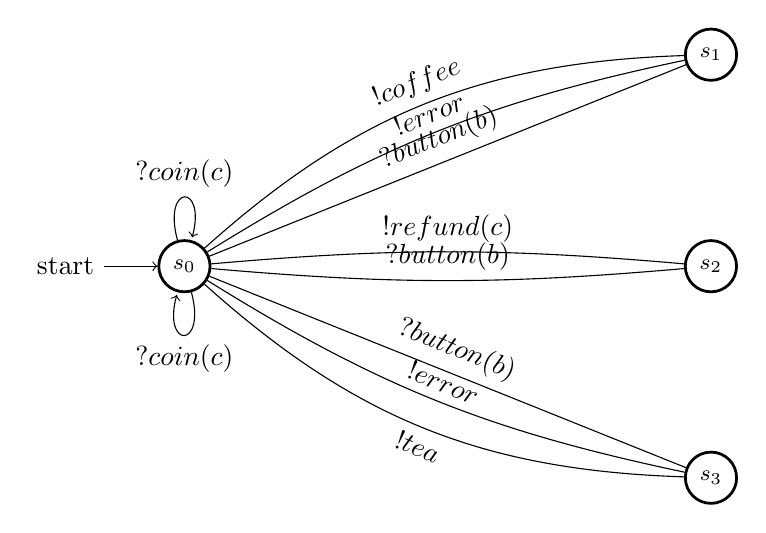
\begin{tikzpicture}[scale=1.5]
	\tikzstyle{every state}=[draw=black,line width=1pt,fill=white,minimum size=5pt]

	\node[state, initial left] (s0) {\footnotesize $s_0$};
  \node[state] (s2) [right=6cm of s0] {\footnotesize $s_2$};
	\node[state] (s1) [above=2cm of s2] {\footnotesize $s_1$};
  \node[state] (s3) [below=2cm of s2] {\footnotesize $s_3$};
	
	\path (s0) edge[min distance=20mm,loop above] node [above] {$?coin(c)$ } (s0) ;
  \path (s0) edge[min distance=20mm,loop below] node [below] {$?coin(c)$ } (s0) ;
	\path (s0) edge node [sloped,midway,above] {$?button(b)$} (s1) ;
  \path (s0) edge[bend right=5] node [sloped,midway,above] {$?button(b)$} (s2) ;
  \path (s0) edge node [sloped,midway,above] {$?button(b)$} (s3) ;
	\path (s1) edge[bend right=20] node [sloped,midway,above] {$!coffee$} (s0) ;
  \path (s1) edge[bend right=10] node [sloped,midway,above] {$!error$} (s0) ;
  \path (s2) edge[bend right=5] node [sloped,midway,above] {$!refund(c)$} (s0) ;
  \path (s3) edge[bend left=20] node [sloped,midway,below] {$!tea$} (s0) ;
  \path (s3) edge[bend left=10] node [sloped,midway,above] {$!error$} (s0) ;
\end{tikzpicture}

\end{figure}
\end{frame}

\begin{frame}{Case study: Coffee machine (9/9)}
\begin{figure}
\input{./figures/cm_sts.tikz}
\end{figure}
\end{frame}

\section[Implementation]{Implementation}

\begin{frame}{Implementation}
\begin{figure}

\usepackage{tikz}     % For graphics
\usepackage{amsmath, amssymb}  % For various math stuff
\usepackage{subfig}
\usepackage{centernot} % For the centernot macro
\usepackage{bbding}

\usetikzlibrary{arrows, automata, shapes.geometric, positioning, backgrounds}

\DeclareMathAlphabet{\mathitbf}{OML}{cmm}{b}{it}

%%%%%%%% COLOURS
\definecolor{darkgreen}{RGB}{0,128,0}


%%%%%%%%%%% HAXXXXORRR

\newenvironment{changemargin}[2]{%
\begin{list}{}{%
\setlength{\topsep}{0pt}%
\setlength{\leftmargin}{#1}%
\setlength{\rightmargin}{#2}%
\setlength{\listparindent}{\parindent}%
\setlength{\itemindent}{\parindent}%
\setlength{\parsep}{\parskip}%
}%
\item[]}{\end{list}}

%%%%%%%%%%%%%%% MATHEMATICAL NOTATIONS%%%%%%%%%
\newcommand{\defi}{\mathrel{{=_{\rm def}}}}
\newcommand{\abs}[1]{\lvert #1 \rvert}
\newcommand{\aut}[1]{\ensuremath{\mathcal{#1}}}
\newcommand{\set}[1]{\{ \, #1 \, \}}
\newcommand{\tuple}[1]{\langle \, #1 \, \rangle}
\newcommand{\suchthat}{\; . \;}
\newcommand{\project}{\mathrel{\upharpoonright}}
\newcommand{\where}{\mid}
\newcommand{\union}{\mathrel{\cup}}
\newcommand{\intersection}{\mathrel{\cap}}
\newcommand{\concat}{\mathrel{\cdot}}
\newcommand{\treq}{\ensuremath{\approx_{\mathrm{tr}} \;}}

\let\oldland\land
\let\oldlor\lor
\let\oldexists\exists
\let\oldforall\forall
\let\oldnexists\nexists

\renewcommand{\land}{\; \oldland \;}
\renewcommand{\lor}{\; \oldlor \;}
\renewcommand{\exists}{\, \oldexists \,}
\renewcommand{\forall}{\, \oldforall \,}
\renewcommand{\nexists}{\, \oldnexists \,}

\newcommand{\existsinfty}{\exists^{\infty}}
\newcommand{\fd}[1]{\ensuremath{\mathit{fd}(#1)}}
\newcommand{\pa}[1]{\ensuremath{\mathit{p}(#1)}}
\newcommand{\qu}[1]{\ensuremath{\mathit{q}(#1)}}
\newcommand{\blockedby}{\nmid}
%%%%%%%%%%%%%%% END MATHEMATICAL NOTATIONS%%%%%%

%%%%%%%%%%%%%%% RULES ETC %%%%%%%%%%%%%%%%%%
\newcounter{ruledefcounter}
\setcounter{ruledefcounter}{1}
\newenvironment{ruledef}[2]%
{\list{}{\leftmargin=0.1in\rightmargin=0in}\item[]\noindent\ignorespaces%
\textbf{Rule R\arabic{ruledefcounter}} %
(#1)%
\textbf{:} %
#2.\list{}{\leftmargin=0.1in\rightmargin=0in}\item[]}
{\endlist\stepcounter{ruledefcounter}\endlist\ignorespacesafterend}
%%%%%%%%%%%%%%% END RULES ETC %%%%%%%%%%%%%%%

%%%%%%%%%%%%%%% THEOREMS ETC %%%%%%%%%%%%%%%
%\theoremstyle{definition}
%\newtheorem{definition}{Definition}[section]
%\theoremstyle{plain}
%\newtheorem{lemma}[definition]{Lemma}
%\newtheorem{proposition}[definition]{Proposition}
%\newtheorem{theorem}[definition]{Theorem}
%\newtheorem{corollary}[definition]{Corollary}
%\theoremstyle{remark}
%\newtheorem{example}[definition]{Example}
%\newtheorem{remark}[definition]{Remark}
%
%\newcommand{\theoremlikeParameterised}[2]{\par\medskip\penalty-250\refstepcounter{definition}{\bfseries\scshape\noindent#1 #2.}\slshape}
%\newenvironment{theoremParam}[1]{\theoremlikeParameterised{\bf Theorem}{#1}}{\par\medskip}
%\newenvironment{lemmaParam}[1]{\theoremlikeParameterised{\bf Lemma}{#1}}{\par\medskip}
%\newenvironment{propositionParam}[1]{\theoremlikeParameterised{\bf Proposition}{#1}}{\par\medskip}
%%%%%%%%%%%%%%% END THEOREMS ETC %%%%%%%%%%%%

%%%%%%%%%%%%%%%% ARROWS %%%%%%%%%%%%%%%%
% auxiliaries
\newcommand{\linefill}{%
   \cleaders
   \hbox{$\smash{\mkern-2mu\mathord-\mkern-2mu}$}%
   \hfill
   \vphantom{\lower1pt\hbox{$\rightarrow$}}%
}

\newcommand{\Linefill}{%
   \cleaders
   \hbox{$\smash{\mkern-2mu\mathord=\mkern-2mu}$}%
   \hfill
   \vphantom{\hbox{$\Rightarrow$}}%
}

% left segment of extensible arrow, no ending
\newcommand{\xleftnoend}[1][]{\mathrel-_{\vphantom{#1}}\mkern-11mu}
\newcommand{\xLeftnoend}[1][]{\mathrel=_{\vphantom{#1}}\mkern-8mu}
% middle segment of extensible arrow
\newcommand{\xmid}[2][]{\stackrel{#2}{\linefill_{\vphantom{#1}}}}
\newcommand{\xMid}[2][]{\stackrel{#2}{\Linefill_{\vphantom{#1}}}}
% right segment of extensible arrow, arrow head
\newcommand{\xrightArrow}[1][]{\mkern-11mu\rightarrow_{#1}}
\newcommand{\xRightArrow}[1][]{\mkern-8mu\Rightarrow_{#1}}
% make arrow symbol
\newcommand{\xmake}[1]{\mathrel{\lower1pt\hbox{$#1$}}}

% single-arrow transition
\newcommand{\trans}[2][]{\xmake{\xleftnoend[#1]\xmid[#1]{#2}\xrightArrow[#1]}}
% negative single-arrow transition
\newcommand{\ntrans}[2][]{\centernot{\trans[#1]{#2}}}
% empty single-arrow transition
\newcommand{\etrans}{\rightarrow}

% double-arrow transition
\newcommand{\Trans}[2][]{\xmake{\xLeftnoend[#1]\xMid[#1]{#2}\xRightArrow[#1]}}
% negative double-arrow transition
\newcommand{\nTrans}[2][]{\centernot{\Trans[#1]{#2}}}
% empty double-arrow transition
\newcommand{\eTrans}{\Rightarrow}
%%%% END ARROWS %%%%%%%%%%%%%%%%%%%%%%%%%

%%%%%%%%%%%%%% TIKZ %%%%%%%%%%%%%%%%
\tikzstyle{background rectangle}= [rounded corners, fill=yellow!20, draw=black, rounded corners=1ex]
\tikzstyle{every picture}=[show background rectangle, ->,>=latex,auto,node distance=1.3cm,thick,initial text=,initial where=above,scale=0.9,transform shape]
\tikzstyle{every state}=[draw=yellow!20,line width=4pt,fill=black,minimum size=5pt]

\tikzstyle{loop right}=[in=-30,out=30,looseness=8]
\tikzstyle{loop left}=[in=150,out=210,looseness=8]
\tikzstyle{loop above}=[in=60,out=120,looseness=8]
\tikzstyle{loop below}=[in=240,out=300,looseness=8]

\tikzstyle{loop above right}=[in=5,out=65,looseness=8]
\tikzstyle{loop above left}=[in=105,out=165,looseness=8]
\tikzstyle{loop slightly above left}=[in=125,out=185,looseness=8]
\tikzstyle{loop slightly above right}=[in=5,out=65,looseness=8]
\tikzstyle{loop below left}=[in=195,out=255,looseness=8]
\tikzstyle{loop below right}=[in=285,out=-15,looseness=8]
\tikzstyle{loop slightly below left}=[in=155,out=215,looseness=8]
\tikzstyle{loop slightly below right}=[in=305,out=5,looseness=8]

\tikzstyle{nodeSmall} = [state, node distance=1.5cm, draw=yellow!20, fill=black]
\tikzstyle{finalNode} = [node distance=1.5cm]
\newcommand{\back}{\color{yellow!20}mm}
\tikzstyle{onEdge}=[fill=yellow!20, pos=0.5]
%%%%%%%%%%%%%% END TIKZ %%%%%%%%%%%%%

%%%%%%%%%%%%%% USEFUL ALIASES %%%%%%%%%
\newcommand{\ioco}{\texttt{ioco}}

\newcommand{\impl}{\aut{A}_i}
\newcommand{\spec}{\aut{A}_s}
\newcommand{\ioconf}{\sqsubseteq_{\ioco}}

\newcommand{\AparB}{\ensuremath{\aut{A} \parallel \aut{B}}}
\newcommand{\AparBie}{\ensuremath{\aut{A} \parallel_{\rm I} \aut{B}}}

\newcommand{\Lin}{L^{\text{\rm I}}}
\newcommand{\Lout}{L^{\text{\rm O}}}
\newcommand{\Ltau}{L^{\tau}}
\newcommand{\Ldelta}{L^{\delta}}
\newcommand{\Ltaudelta}{L^{\delta}_{\tau}}
\newcommand{\LA}{L_{\aut{A}}}
\newcommand{\LB}{L_{\aut{B}}}
\newcommand{\LC}{L_{\aut{C}}}
\newcommand{\LD}{L_{\aut{D}}}
\newcommand{\LinA}{\Lin_{\aut{A}}}
\newcommand{\LinB}{\Lin_{\aut{B}}}
\newcommand{\LinC}{\Lin_{\aut{C}}}
\newcommand{\LinD}{\Lin_{\aut{D}}}
\newcommand{\LoutA}{\Lout_{\aut{A}}}
\newcommand{\LoutB}{\Lout_{\aut{B}}}
\newcommand{\LoutC}{\Lout_{\aut{C}}}
\newcommand{\LoutD}{\Lout_{\aut{D}}}
\newcommand{\LoutHide}{\Lout_{H}}
\newcommand{\LtauA}{\Ltau_{\aut{A}}}
\newcommand{\LtauB}{\Ltau_{\aut{B}}}
\newcommand{\LtauC}{\Ltau_{\aut{C}}}
\newcommand{\LtauD}{\Ltau_{\aut{D}}}
\newcommand{\LtauHide}{\Ltau_{H}}
\newcommand{\LdeltaA}{\Ldelta_{\aut{A}}}
\newcommand{\LdeltaB}{\Ldelta_{\aut{B}}}
\newcommand{\LdeltaC}{\Ldelta_{\aut{C}}}
\newcommand{\LdeltaD}{\Ldelta_{\aut{D}}}
\newcommand{\LAparB}{L_{\AparB}}
\newcommand{\LinAparB}{\Lin_{\AparB}}
\newcommand{\LoutAparB}{\Lout_{\AparB}}
\newcommand{\LtauAparB}{\Ltau_{\AparB}}
\newcommand{\LdeltaAparB}{\Ldelta_{\AparB}}

\newcommand{\sdelta}{s_{\delta}}
\newcommand{\fdelta}{f_{\delta}}

\newcommand{\SA}{S_{\aut{A}}}
\newcommand{\SB}{S_{\aut{B}}}
\newcommand{\SC}{S_{\aut{C}}}
\newcommand{\SD}{S_{\aut{D}}}
\newcommand{\SAparB}{S_{\AparB}}
\newcommand{\Sdelta}{S_{\delta}}
\newcommand{\Shide}{S_{H}}

\newcommand{\Sstart}{S^0}
\newcommand{\SstartA}{\Sstart_{\aut{A}}}
\newcommand{\SstartB}{\Sstart_{\aut{B}}}
\newcommand{\SstartC}{\Sstart_{\aut{C}}}
\newcommand{\SstartD}{\Sstart_{\aut{D}}}
\newcommand{\SstartAparB}{\Sstart_{\AparB}}

\newcommand{\PA}{P_{\aut{A}}}
\newcommand{\PB}{P_{\aut{B}}}
\newcommand{\PC}{P_{\aut{C}}}
\newcommand{\PD}{P_{\aut{D}}}
\newcommand{\PAparB}{P_{\AparB}}

\newcommand{\transA}[2][]{\trans[#1]{#2}_{\aut{A}}}
\newcommand{\transB}[2][]{\trans[#1]{#2}_{\aut{B}}}
\newcommand{\transC}[2][]{\trans[#1]{#2}_{\aut{C}}}
\newcommand{\transD}[2][]{\trans[#1]{#2}_{\aut{D}}}
\newcommand{\transAparB}[2][]{\trans[#1]{#2}_{\AparB}}
\newcommand{\transAparBie}[2][]{\trans[#1]{#2}_{\AparBie}}
\newcommand{\transDelta}[2][]{\trans[#1]{#2}_{\delta}}
\newcommand{\transDet}[2][]{\trans[#1]{#2}_{\mathrm{D}}}
\newcommand{\transHide}[2][]{\trans[#1]{#2}_{H}}
\newcommand{\transDeltaHide}[2][]{\trans[#1]{#2}_{\delta(\mathrm{H})}}
\newcommand{\transHideDelta}[2][]{\trans[#1]{#2}_{\mathrm{H}(\delta)}}

\newcommand{\TransA}[2][]{\Trans[#1]{#2}_{\aut{A}}}
\newcommand{\TransB}[2][]{\Trans[#1]{#2}_{\aut{B}}}
\newcommand{\TransC}[2][]{\Trans[#1]{#2}_{\aut{C}}}
\newcommand{\TransD}[2][]{\Trans[#1]{#2}_{\aut{D}}}
\newcommand{\TransAparB}[2][]{\Trans[#1]{#2}_{\AparB}}
\newcommand{\TransAparBie}[2][]{\Trans[#1]{#2}_{\AparBie}}
\newcommand{\TransDelta}[2][]{\Trans[#1]{#2}_{\delta}}
\newcommand{\TransDet}[2][]{\Trans[#1]{#2}_{\mathrm{D}}}
\newcommand{\TransHide}[2][]{\Trans[#1]{#2}_{H}}
\newcommand{\TransHideDelta}[2][]{\Trans[#1]{#2}_{\mathrm{H}(\delta)}}

\newcommand{\ntransA}[2][]{\ntrans[#1]{#2}_{\aut{A}}}
\newcommand{\ntransB}[2][]{\ntrans[#1]{#2}_{\aut{B}}}
\newcommand{\ntransC}[2][]{\ntrans[#1]{#2}_{\aut{C}}}
\newcommand{\ntransD}[2][]{\ntrans[#1]{#2}_{\aut{D}}}
\newcommand{\ntransAparB}[2][]{\ntrans[#1]{#2}_{\AparB}}
\newcommand{\ntransAparBie}[2][]{\ntrans[#1]{#2}_{\AparBie}}
\newcommand{\ntransDelta}[2][]{\ntrans[#1]{#2}_{\delta}}
\newcommand{\ntransHide}[2][]{\ntrans[#1]{#2}_{H}}
\newcommand{\ntransDet}[2][]{\ntrans[#1]{#2}_{\mathrm{D}}}

\newcommand{\nTransA}[2][]{\nTrans[#1]{#2}_{\aut{A}}}
\newcommand{\nTransB}[2][]{\nTrans[#1]{#2}_{\aut{B}}}
\newcommand{\nTransC}[2][]{\nTrans[#1]{#2}_{\aut{C}}}
\newcommand{\nTransD}[2][]{\nTrans[#1]{#2}_{\aut{D}}}
\newcommand{\nTransAparB}[2][]{\nTrans[#1]{#2}_{\AparB}}
\newcommand{\nTransAparBie}[2][]{\nTrans[#1]{#2}_{\AparBie}}
\newcommand{\nTransDelta}[2][]{\nTrans[#1]{#2}_{\delta}}
\newcommand{\nTransDet}[2][]{\nTrans[#1]{#2}_{\mathrm{D}}}
\newcommand{\nTransHide}[2][]{\nTrans[#1]{#2}_{H}}

\newcommand{\etransA}{\etrans_{\aut{A}}}
\newcommand{\etransB}{\etrans_{\aut{B}}}
\newcommand{\etransC}{\etrans_{\aut{C}}}
\newcommand{\etransD}{\etrans_{\aut{D}}}
\newcommand{\etransAparB}{\etrans_{\AparB}}
\newcommand{\etransAparBie}{\etrans_{\AparBie}}
\newcommand{\etransDelta}{\etrans_{\delta}}
\newcommand{\etransDet}{\etrans_{\mathrm{D}}}
\newcommand{\etransHide}{\etrans_{H}}
\newcommand{\etransDeltaHide}{\etrans_{\delta(\mathrm{H})}}
\newcommand{\etransHideDelta}{\etrans_{\mathrm{H}(\delta)}}

\newcommand{\deltaf}[1]{\ensuremath{\delta(#1)}}
\newcommand{\deter}[1]{\ensuremath{\mathit{det}(#1)}}
\newcommand{\hide}[2]{\ensuremath{#1 \setminus #2}}
\newcommand{\init}[1]{\ensuremath{\mathit{init}(#1)}}
\newcommand{\trace}[1]{\ensuremath{\mathit{trace}(#1)}}
\newcommand{\states}[1]{\ensuremath{\mathit{states}(#1)}}
\newcommand{\paths}[1]{\ensuremath{\mathit{paths}(#1)}}
\newcommand{\dpaths}[1]{\ensuremath{\mathit{dpaths}(#1)}}
\newcommand{\fpaths}[1]{\ensuremath{\mathit{fpaths}(#1)}}
\newcommand{\fdpaths}[1]{\ensuremath{\mathit{fdpaths}(#1)}}

\newcommand{\rs}[1]{\ensuremath{\mathit{rs}_{#1}}}
\newcommand{\qos}[1]{\ensuremath{\mathit{qos}_{#1}}}

\newcommand{\fdclosures}[1]{\ensuremath{\mathit{fdclosures}(#1)}}
\newcommand{\newfdclosures}[1]{\ensuremath{\mathit{new\text{-}fdclosures}(#1)}}

\newcommand{\reach}[1]{\ensuremath{\mathit{reach}(#1)}}
\newcommand{\reachA}[1]{\ensuremath{\mathit{reach}_{\aut{A}}(#1)}}
\newcommand{\reachB}[1]{\ensuremath{\mathit{reach}_{\aut{B}}(#1)}}
\newcommand{\reachAparB}[1]{\ensuremath{\mathit{reach}_{\AparB}(#1)}}
\newcommand{\reachHide}[1]{\ensuremath{\mathit{reach}_{H}(#1)}}

\newcommand{\traces}[1]{\ensuremath{\mathit{traces}(#1)}}
\newcommand{\tracesA}[1]{\ensuremath{\mathit{traces}_{\aut{A}}(#1)}}
\newcommand{\tracesB}[1]{\ensuremath{\mathit{traces}_{\aut{B}}(#1)}}
\newcommand{\tracesAparB}[1]{\ensuremath{\mathit{traces}_{\AparB}(#1)}}
\newcommand{\tracesDelta}[1]{\ensuremath{\mathit{traces}_{\delta}(#1)}}
\newcommand{\tracesDet}[1]{\ensuremath{\mathit{traces}_{\mathrm{D}}(#1)}}
\newcommand{\tracesHide}[1]{\ensuremath{\mathit{traces}_{H}(#1)}}
\newcommand{\tracesDeltaHide}[1]{\ensuremath{\mathit{traces}_{\delta(\mathrm{H})}(#1)}}
\newcommand{\tracesHideDelta}[1]{\ensuremath{\mathit{traces}_{\mathrm{H}(\delta)}(#1)}}
%%%%%%%%%%% END USEFUL ALIASES  %%%%%%%%%

\begin{tikzpicture}
\node (GROOVE) {
  \includegraphics[scale=0.08]{./figures/groove.png}
};
\node (GROOVE TAG) [below=1pt of GROOVE]{\textbf{GROOVE}};
\node (GG2STS) [shape = rectangle, fill = black!30!white, below right=-5pt and -5pt of GROOVE]{\textbf{GG -> STS}};
\node (Cloud) [above right=3cm and 1cm of GROOVE] {
  \includegraphics[]{./figures/cloud.png}
};
\node (ATM) [right=5cm of GROOVE] {
  \includegraphics[scale=0.08]{./figures/atm.png}
};
\node (ATM TAG) [below=1pt of ATM]{\textbf{ATM}};

\node (SUT) [above=1.5cm of ATM] {
  \includegraphics[scale=0.10]{./figures/coffee_machine.jpg}
};

\path ([xshift=2ex]ATM.north) edge node [sloped,midway,above] {input} ([xshift=2ex]SUT.south) ;
\path ([xshift=-2ex]SUT.south) edge node [sloped,midway,above] {output}  ([xshift=-2ex]ATM.north) ;

\path (GROOVE) edge node [sloped,midway,above] {STS}(Cloud) ;
\path (Cloud) edge node [sloped,midway,above] {STS} (ATM) ;
\end{tikzpicture}
\end{figure}
\end{frame}

\section[Validation]{Validation}

\begin{frame}{Model Examples}
\begin{itemize}
  \item 5 example cases used:
  \begin{enumerate}
    \item a boardgame
    \item a puzzle
    \item a reservation system
    \item a bar tab system
    \item a self-checkout register
  \end{enumerate}
  \item Model examples with Graph Grammar and STS
  \item Compare models
\end{itemize}
\end{frame}

\begin{frame}{Measurements}
  \begin{itemize}
  \item Performance (How fast does GRATiS make STS?)
  \item Simulation (Does the STS built by GRATiS express the same behavior as the modelled STS?)
  \item Redundancy (Is the STS built by GRATiS larger than the modelled STS?)
  \item Model complexity (Is there a difference in complexity between the STS and the Graph Grammar?)
  \item Extendability (How easy is it to adapt both models to a hypothetical extension?)
  \end{itemize}
\end{frame}

\begin{frame}{Measurement conclusions}
  \begin{itemize}
  \item Performance: less than 10 seconds for large case study
  \item Simulation: No problems found
  \item Redundancy: Technique can create redundant STSs
  \item Model complexity: Both are equally complex
  \item Extendability: Varying results
  \end{itemize}
\end{frame}

\section[Conclusion]{Conclusion}

\begin{frame}{Conclusion}
  \begin{itemize}
    \item Created method of generating STSs from Graph Grammars
    \item Implemented a tool for model-based testing with Graph Grammars
    \item Validated the tool using case studies
    \item Showed modelling behavior with Graph Grammars is effective
  \end{itemize}
\end{frame}

\end{document}
